\documentclass[compress]{beamer}
\mode<presentation>
\setbeamercovered{transparent}
\usetheme{Warsaw}
%\useoutertheme{smoothtree}
\usepackage{multirow}
\usepackage[english]{babel}
\usepackage[latin1]{inputenc}
\usepackage{times}
\usepackage[T1]{fontenc}
\usepackage{xmpmulti}
\usepackage{multicol}
\usepackage{colortbl}

%\setbeamersize{text margin left=.25 in,text margin right=.25 in}
\setbeamersize{text margin left=.15 in,text margin right=.15 in}
\usepackage[authoryear]{natbib}


\usepackage{epstopdf}
\usepackage{xcolor}
\usepackage{latexcolors}
%\usepackage[dvipsnames]{xcolor}
\definecolor{antiquebrass}{rgb}{0.8, 0.58, 0.46}
\definecolor{babyblueeyes}{rgb}{0.63, 0.79, 0.95}
\definecolor{babyblue}{rgb}{0.54, 0.81, 0.94}
\definecolor{bistre}{rgb}{0.24, 0.17, 0.12}
\definecolor{brightlavender}{rgb}{0.75, 0.58, 0.89}
\definecolor{bulgarianrose}{rgb}{0.28, 0.02, 0.03}
\definecolor{slateblue}{rgb}{0.56, 0.74, 0.56}
\definecolor{cordovan}{rgb}{0.54, 0.25, 0.27}
\definecolor{darkbyzantium}{rgb}{0.36, 0.22, 0.33}

\setbeamercolor{structure}{fg=babyblue!100, bg= black!60}







\usepackage{tikz}
\usetikzlibrary{shadows,calc}
\usetikzlibrary{shadows.blur}
\usetikzlibrary{shapes.symbols}
\usepackage{hyperref}
\usepackage{booktabs}
\usepackage{colortbl}
\usepackage{multirow}
%%%%%%%%% shaddow image %%%%%
% some parameters for customization
\def\shadowshift{3pt,-3pt}
\def\shadowradius{6pt}
\colorlet{innercolor}{black!60}
\colorlet{outercolor}{gray!05}
% this draws a shadow under a rectangle node
\newcommand\drawshadow[1]{
\begin{pgfonlayer}{shadow}
    \shade[outercolor,inner color=innercolor,outer color=outercolor] ($(#1.south west)+(\shadowshift)+(\shadowradius/2,\shadowradius/2)$) circle (\shadowradius);
    \shade[outercolor,inner color=innercolor,outer color=outercolor] ($(#1.north west)+(\shadowshift)+(\shadowradius/2,-\shadowradius/2)$) circle (\shadowradius);
    \shade[outercolor,inner color=innercolor,outer color=outercolor] ($(#1.south east)+(\shadowshift)+(-\shadowradius/2,\shadowradius/2)$) circle (\shadowradius);
    \shade[outercolor,inner color=innercolor,outer color=outercolor] ($(#1.north east)+(\shadowshift)+(-\shadowradius/2,-\shadowradius/2)$) circle (\shadowradius);
    \shade[top color=innercolor,bottom color=outercolor] ($(#1.south west)+(\shadowshift)+(\shadowradius/2,-\shadowradius/2)$) rectangle ($(#1.south east)+(\shadowshift)+(-\shadowradius/2,\shadowradius/2)$);
    \shade[left color=innercolor,right color=outercolor] ($(#1.south east)+(\shadowshift)+(-\shadowradius/2,\shadowradius/2)$) rectangle ($(#1.north east)+(\shadowshift)+(\shadowradius/2,-\shadowradius/2)$);
    \shade[bottom color=innercolor,top color=outercolor] ($(#1.north west)+(\shadowshift)+(\shadowradius/2,-\shadowradius/2)$) rectangle ($(#1.north east)+(\shadowshift)+(-\shadowradius/2,\shadowradius/2)$);
    \shade[outercolor,right color=innercolor,left color=outercolor] ($(#1.south west)+(\shadowshift)+(-\shadowradius/2,\shadowradius/2)$) rectangle ($(#1.north west)+(\shadowshift)+(\shadowradius/2,-\shadowradius/2)$);
    \shade[outercolor,right color=innercolor,left color=innercolor] ($(#1.north west)+(-\shadowradius/12,\shadowradius/12)$) rectangle ($(#1.south east)+(\shadowradius/12,-\shadowradius/12)$);%Frame
    \filldraw ($(#1.south west)+(\shadowshift)+(\shadowradius/2,\shadowradius/2)$) rectangle ($(#1.north east)+(\shadowshift)-(\shadowradius/2,\shadowradius/2)$);
\end{pgfonlayer}
}
% create a shadow layer, so that we don't need to worry about overdrawing other things
\pgfdeclarelayer{shadow} 
\pgfsetlayers{shadow,main}
% Define image shadow command
\newcommand\shadowimage[2][]{%
\begin{tikzpicture}
\node[anchor=south west,inner sep=0] (image) at (0,0) {\includegraphics[#1]{#2}};
\drawshadow{image}
\end{tikzpicture}}
\usepackage{calligra}

\DeclareMathOperator*{\argmax}{Arg\,max}
\DeclareMathOperator*{\argmin}{Arg\,min}
\newcommand{\norm}[1]{\left\Vert #1 \right\Vert }
\newcommand{\bbetaHat}{ \widehat{\bbeta}}
\newcommand{\bbetaLSE}{ \widehat{\bbeta}_{_{\text{LSE}}}}
\newcommand{\bbetaMLE}{ \widehat{\bbeta}_{_{\text{MLE}}}}
\newcommand{\sqBullet}[1]{  {\tiny \tiny \tiny \qBoxCol{#1!60}{ }} }
%***************
%\newtheorem{thm}{Theorem}
%\documentclass[noinfoline]{imsart}
%\usepackage{amsmath,amstext,amssymb}
%%\usepackage[top=1.5in, bottom=1.5in, left=1.2in, right=1.2in]{geometry}
%% settings
%%\pubyear{2005}
%%\volume{0}
%%\issue{0}
%%\firstpage{1}
%%\lastpage{8}
%\arxiv{arXiv:0000.0000}

%\startlocaldefs
%\numberwithin{equation}{section}
%\theoremstyle{plain}
%\newtheorem{thm}{Theorem}
%\endlocaldefs
\usepackage{lipsum} 
\usepackage{amsmath}
\usepackage{amssymb}
\usepackage{amsbsy} 
\usepackage{amsthm}
\usepackage{mathrsfs}
\usepackage{eufrak}
\usepackage{mathrsfs}
\usepackage{color}
\usepackage{verbatim}
\usepackage{graphicx}
\usepackage{bm}
\usepackage{enumerate}
\usepackage{epstopdf} 
\usepackage{natbib}
\usepackage{undertilde}
%\RequirePackage[colorlinks,citecolor=blue,urlcolor=blue]{hyperref}
%\usepackage{subfig}
\usepackage[final]{pdfpages}

\usepackage{algorithm}  %@subhajit
\usepackage{algpseudocode} %@subhajit
\usepackage{algorithmicx}     %@subhajit
\usepackage{undertilde}


\newcommand{\sphere}{{\mathbb{S}}}
\newcommand{\R}{\mathbb{R}}
\newcommand{\LatentV}{V}
\newcommand{\NC}{m}
\newcommand{\Priorf}{f_{prior}}
\newcommand{\FWOne}[2]{{{}_{1}\Psi _{1}\left[{\begin{matrix}(\frac{#1}{2},\frac{1}{2})\\(1,0)\end{matrix}};#2\right]} 
}


\newcommand{\HyPriorMu}{\thetabf}
\newcommand{\HyPriorAlpha}{\alpha}
\newcommand{\HyPriorBeta}{\beta}
\newcommand{\HyPriorK}{\zeta}
\newcommand{\Indicator}[2]{\mathbb{I}_{_{#1}}({#2 })}
\newcommand{\xb}{\bm{x}}
\newcommand{\bx}{\MakeVec{\bm{x}}}
\newcommand{\bX}{\bm{X}}
\newcommand{\by}{\MakeVec{\bm{y}}}
\newcommand{\bZ}{\bm{Z}}
\newcommand{\bF}{\bm{F}}
\newcommand{\btheta}{\MakeVec{{\bm{\theta}}}}
\newcommand{\Bpi}{\MakeVec{\boldsymbol{\pi}}}
\newcommand{\thetabf}{\MakeVec{\boldsymbol{\theta}}}
\newcommand{\Thetabf}{\boldsymbol{\Theta}}
\newcommand{\taubf}{\MakeVec{\boldsymbol{\tau}}}
\newcommand{\Tr}{Tr}


\newcommand{\bM}{\bm{M}}
\newcommand{\bD}{\MakeVec{\bm{D}}}
\newcommand{\bV}{\MakeVec{\bm{V}}}
\newcommand{\loglikmix}{\mathcal{L}_{\bM,\bD,\bV}}
\newcommand{\hypdc}{{}_0F_1\left(\frac{n}{2},\frac{D_c^2}{4}\right)}


\usepackage{xstring}
\usepackage[normalem]{ulem}
\definecolor{ultramarine}{RGB}{38,29,163}
\newcommand\PalDel[1]{{\color{red} {\sout{#1}}}}
\newcommand\Pal[1]{{\color{ultramarine}{#1}}}
\newcommand\PalRp[2]{\PalDel{#1} \Pal{#2}}
\newcommand\PalCmnt[1]{{\color{ultramarine} {[[[***PAL:  #1 ***]]]}}}

\newcommand{\qedwhite}{\hfill \ensuremath{\Box}}
\newcommand{\SpaceD}{\mathcal{S}_p}
\newcommand{\SpaceM}{\widetilde{\mathcal{V}}_{n,p}}
\newcommand{\SpaceV}{\mathcal{V}_{p,p}}
\newcommand{\SpaceF}{\mathbb{R}^{n,p}}
\newcommand{\StiefelS}{\mathcal{V}_{n,p}}
\newcommand{\SpacePi}{\mathbb{S}_{\pi}}
\newcommand{\ML}{{\cal{ML}}}
\newcommand{\ProdSpace}{\boldsymbol{\Theta}}
\newcommand{\ThetaAndPi}{\Xi}
\newcommand{\ClassML}{\mathcal{C}_{\ML}}


\newcommand{\balpha}{\MakeVec{\bm{\alpha}}}
\newcommand{\bbeta}{\MakeVec{\bm{\beta}}}
\newcommand{\bEta}{\bm{\eta}}
\newcommand{\bd}{{\utilde{\bm{d}}}}
\newcommand{\BoEta}{{\utilde{\boldsymbol{\eta}}}}
%\newtheorem{theorem}{Theorem}[section]
%\newtheorem{theorem}{Theorem}
%\newtheorem{lemma}{Lemma}
%\newtheorem{result}{Result}
\newtheorem{defn}{Definition}
\newcommand{\pdv}[2][]{\frac{\partial#1}{\partial#2}}
\newcommand{\pdvtwo}[2][]{\frac{\partial^2#1}{{\partial#2}^2}}


%\newcommand{\mubf}{\boldsymbol{\mu}}
\newcommand{\mubf}{\MakeVec{\mu}}
\newcommand{\sumI}{ \sum_{i=1}^{n}}
\newcommand{\Ybar}{{\overline{Y}}}

\newcommand{\Expectation}[1]{\mathbb{E}{[#1]}}
\newcommand{\priorXzero}{\Psi}
\newcommand{\iMat}{\mathbf{I}_{p}}

% 
% \newtheorem{thm}{Theorem}[section]
% \newtheorem{cor}[thm]{Corollary}
% \newtheorem{lem}[thm]{Lemma}
%\newtheorem{proposition}{Proposition}

%\newtheorem{theorem}{Theorem}[chapter]%To link the theorem to each chapter uncomment the chapter option
%\newtheorem{lemma}{Lemma}%[theorem]% To link each lemma to a theorem uncomment the theorem option
%\newtheorem{corollary}{Corollary}%[theorem]% To link each corollary to a theorem uncomment the theorem option
% to link a corollary to a chapter change the theorem option to chapter
%\newtheorem{definition}{Definition}%[chapter] %the same is true for both definitions and assumptions
\newtheorem{assumption}{Assumption}%[chapter] %
%\newtheorem{proposition}{Proposition}[chapter]
%\newtheorem{fact}{Fact} %%% added by @subho
\newcommand{\StrongNBD}[2]{S_{#1}{#2}}
\newcommand{\bpi} {\boldsymbol{\pi}}
\newcommand{\bphi} {\boldsymbol{\phi}}
\newcommand{\bb}[1]{\boldsymbol{#1}}
% Definitions of handy macros can go here

\newcommand{\normtwo}[1]{{\left\lVert#1\right\rVert}_2}

\newcommand{\dataset}{{\cal D}}
\newcommand{\fracpartial}[2]{\frac{\partial #1}{\partial  #2}}
\newcommand{\Lesbegue}[1]{\mu_{\btheta_{#1},\bpi_{#1}}}
\newcommand{\fthetapi}[1]{f_{\btheta_{#1},\bpi_{#1}}}
% Heading arguments are {volume}{year}{pages}{submitted}{published}{author-full-names}
\newcommand{\doublehat}[1]{%
    \settoheight{\dhatheight}{\ensuremath{\widehat{#1}}}%
    \addtolength{\dhatheight}{-0.35ex}%
    \widehat{\vphantom{\rule{2pt}{\dhatheight}}%
    \smash{\hspace{-0.5mm}\widehat{#1}}}}

\newcommand{\hyp}{{}_0F_1\left(\frac{n}{2},\frac{D^2}{4}\right)}
\newcommand{\hypinline}{{}_0F_1\left({n}/{2},{D^2}/{4}\right)}

\newcommand{\partialhyp}[1]{\frac{\partial}{\partial\,{d_{#1}}}\,\left[\hyp\right]}

\newcommand{\fracProbZ}[1]{\frac{\langle Z_{ic} \rangle \, #1}{\sum_{i=1}^{N} \langle Z_{ic}\rangle  } }
\newcommand{\EmVar}[1]{\widetilde{#1}^{(c)}}

\newcommand{\IMDY}{{\it{CCPD}}}
\newcommand{\JMDY}{{\it{JCPD}}}

\newcommand{\DYlang}{\frac{\exp(\nu\,\bEta^T\bd)}{{\left[{}_0F_1\left(\frac{n}{2},\frac{D^2}{4}\right)\right]}^{\nu}}}

\newcommand{\logDYlang}{\nu\,\bEta^T\bd - \nu\,\log\left({}_0F_1\left(\frac{n}{2},\frac{D^2}{4}\right)\right)}

\newcommand{\lhyp}{\log\left({}_0F_1\left(\frac{n}{2},\frac{D^2}{4}\right)\right)}

%\jmlrheading{1}{2000}{1-48}{4/00}{10/00}{SS \& JH \& AB}

% Short headings should be running head and authors last names

%\ShortHeadings{BDP and cIBP}{SS \& JH \& AB}
%\firstpageno{1}

\newcommand{\diam}[1]{{{#1}^{\ast}}}

%%% coloring option %%%
\definecolor{auburn}{rgb}{0.53, 0.1, 0.5}
\newcommand{\sss}{\color{auburn}}  %%% for Subhajit
\newcommand{\sse}{\color{black}}
\newcommand{\attn}{\color{red}}
\newcommand{\rms}{\color{magenta}}  %%% for Riten
\newcommand{\rme}{\color{black}}
\newcommand{\MLDensity}{f_{\ML}}
\setlength{\parindent}{0cm}
\newcommand{\posterior}

\newcommand{\variableX}{\bd}
\newcommand{\funch}{\mathfrak{h}}
\newcommand{\IndVzero}[1]{\mathbb{I}({X\in \mathcal{V}^{#1}_0})}
\newcommand{\Rnp}{\mathbb{R}^{n \times p}}
\newcommand{\Rpp}{\mathbb{R}^{p \times p}}
\newcommand{\vecnorm}[1]{\lVert #1\rVert}

\newcommand{\etapsiD}{\eta_{\priorXzero}}
\newcommand{\BoEtapsiD}{\BoEta_{\priorXzero}}

\newcommand{\DMp}{\mathcal{D}^{p \times p}}
\newcommand{\Rplus}{\mathbb{R}_{+}}
\newcommand{\prodMeasure}{\Upsilon}

\newcommand{\m}{{\bf m_{\BoEta}}} 
\newcommand{\SetWithMode}{\mathcal{S}}
\newcommand{\SetWithModePrime}{\mathcal{S}}
\newcommand{\TargetComp}{\mathcal{S}^{\star}}

\newcommand{\ConstCondDen}{K_{\nu, \BoEta}} 

\newcommand{\hyparam}[2]{
    \IfEqCase{#1}{
        {M}{\xi^{#2}_c}
        {V}{\gamma^{#2}_c}%
        
    }
  }
\newcommand{\threepartdef}[6]
{
	\left\{
		\begin{array}{lll}
			#1 & \mbox{if } #2 \\
			#3 & \mbox{if } #4 \\
			#5 & \mbox{if } #6
		\end{array}
	\right.
}

\def\bv{\color{blue}}
\def\ev{\color{black}}
\newcommand{\bch}{\bv }
\newcommand{\ech}{\ev\normalsize}
%\newcommand{\MakeVec}[1]{{\utilde{\bf #1}}}
\newcommand \Measure[2][]{%
  \ifstrempty{#1}{
  \IfEqCase{#2}{
        {M}{\mu}%
        {D}{\mu_1}%
        {V}{\mu_2}
        {X}{\mu}
   }  
  }{
  \IfEqCase{#1}{
  {1}{
   \IfEqCase{#2}{
        {M}{d\mu(M)}%
        {D}{d\mu_1(\bd)}%
        {V}{d\mu_2(V)}
        {X}{d\mu(X)}
        {Y}{d\mu(Y)}
        {MDV} {d\mu(M)\; d\mu_1(\bd) \;d\mu_2(V) }
        }
   } 
   {2}{
   \IfEqCase{#2}{
         {M}{d\mu(M^{\ast})}%
        {D}{d\mu_1(\bd^{\ast})}%
        {V}{d\mu_2(V^{\ast})}
        {X}{d\mu(X^{\ast})}
        }
   }
   {3}{
   \IfEqCase{#2}{
         {M}{\mu(dM^{\star})}%
        {D}{\mu_2(d\bd^{\star})}%
        {V}{\mu_1(dV^{\star})}
        {X}{\mu(X^{\star})}
        }
   }   
   
   } 
  }%
}
  \newcommand{\VONF}{\text{VonMisesFisher}}
\newcommand{\MPGalpha}{\alpha}
\newcommand{\MPGnu}{\nu}
\newcommand{\MPG}{MPG }
\newcommand{\ybin}{y^{(\text{bin})}}


%\newcommand{\abs}[1]{\left \vert  #1  \right\vert  }
\usepackage{caption}
\usepackage{subcaption}

%%%%%%%%%%%%%%%%%%%%%%%%%%%
\newcommand{\IEHC}{\text{IEHC}}







\newcommand \Th[1]{%
  \IfEqCase{#1}{
        {1}{ 1^{\text{st}}}%
        {2}{2^{\text{nd}}}%
        {3}{3^{\text{rd}}}%
  }[{#1}^{\text{th}}]
}
  
  
   \newcommand{\augV}{\text{aux}}
  
  
  
  
  \newcommand{\CDE}{\text{PL}}
\newcommand{\CDEsigma}{\sigma}
\newcommand{\CDEepsilon}{\SVepsilon}
\newcommand{\CDEmu}{\mu}
 % \newcommand{\SVepsilon}{\varepsilon}
  \newcommand{\SVepsilon}{\delta}
 \newcommand{\abs}[1]{\left\lvert{#1}\right \rvert }
 
 
\newcommand{\CPDX }{\text{CPDX}}
\newcommand{\CPDXPar}{\vartheta}
\newcommand{\K}{\mathcal{K}}



\newcommand{\lossFunctionOne}[1]{ \left\{ \abs{ ( \abs{#1}-\SVepsilon)}  + ( \abs{#1}-\SVepsilon)\right\} }

\newcommand{\lossFunctionAlt}[1]{ \abs{  #1-\SVepsilon}  + \abs{ #1+\SVepsilon}-2\SVepsilon }

\newcommand{\lossFunctionAltOne}[1]{   \lossFunctionAlt{ \frac{\left(#1\right)}{\sigma}}}

\newcommand{\lossFunction}[1]{ \left\{ \abs{ \left( \frac{\abs{#1}}{\sigma}-\SVepsilon\right)}  + \left( \frac{\abs{#1}}{\sigma}-\SVepsilon\right)\right\} }
\newcommand{  \Likelihood}{\mathcal{L}}
%\newcommand{\Onebf}{\bf 1}
\newcommand{\Onebf}{{\bf \utilde{1}_{n}}}





\newcommand{\InvGamma}{\text{InvGamma}}
\newcommand{\PriorSigmaAlpha}{a}
\newcommand{\PriorSigmaBeta}{b}
\newcommand{\PriorBetaMean}{\mubf_{_{\bbeta}}}
\newcommand{\PriorBetaVar}{\Sigma_{_{\bbeta}}  }
\newcommand{\mvnormPdf}[4]{\frac{1}{ \left({2\pi}\right)^{\frac{#4}{2}} \sqrt{\vert{#3}\vert}}{\exp\left[ - \frac{1}{2}(#1- #2)^T {#3}^{-1} (#1- #2)\right]}      }
\newcommand{\InvGammaPdf}[3]{ \frac{(#1)^{-#2+1}}{\Gamma\left( #2\right) } \exp\left[ -\frac{{#3}}{{#1}} \right] }

 \newcommand{\byTilde}{\tilde{\by}}
 
 \newcommand{\TrfSigma}{\varsigma}
 \newcommand{ \Normal}{\text{Normal}}
 \newcommand{\GlobalPar}{\tau}
\newcommand{\LocalPar}{\psi}
\newcommand{\Not}[1]{{\overline{#1}}}
\newcommand{\st}{:}

\newcommand{\define}[2]{ \begin{definition}[#1]  #2  \end{definition}  }

\newcommand{\Exmpl}[2]{\qBrd[0.75in]{#1}{Example #2:}}
\newcommand{\Qn}{\HLTW{Question:} }


\newcommand{\pmf}{p}
\newcommand{\cdf}{F}
%\NewDocumentCommand{\support}{O{ }}{{\mathcal{S}}_{_{#1}}}
\NewDocumentCommand{\support}{O{ }}{{\mathbb{S}}_{_{#1}}}
%\newcommand{\SampleS}{\mathcal{S}}
\newcommand{\SampleS}{\mathscr{S}}
\usepackage{xcolor}
\usepackage{xparse}
\definecolor{lightGray}{gray}{0.95}
\definecolor{lightGrayOne}{gray}{0.9}
\definecolor{lightBlueOne}{RGB}{204, 255, 255}
\definecolor{lightBlueTwo}{RGB}{204, 238, 255}
\definecolor{lightBlueThree}{RGB}{204, 204, 255}
\definecolor{AltBlue}{RGB}{119,14,161}
\definecolor{Orchid}{RGB}{186,85,211}

\definecolor{BGBlue}{RGB}{220,221,252}
\definecolor{BGBlueOne}{RGB}{204,229,255}

\definecolor{DarkGreenOne}{RGB}{34,139,34}

\definecolor{BGGreen}{RGB}{240,243,245}
\definecolor{lightGreenOne}{RGB}{179, 255, 179}
\definecolor{lightGreenTwo}{RGB}{198, 255, 179}
\definecolor{lightGreenThree}{RGB}{243, 255, 230}
\definecolor{AltGreen}{RGB}{193, 240, 240}

\definecolor{BOGreen}{RGB}{180,0,0}
\definecolor{BGGreenOne}{RGB}{220,250,220}

\definecolor{lightBrownOne}{RGB}{255, 221, 204}
\definecolor{lightBrownTwo}{RGB}{255, 229, 204}
\definecolor{lightBrownThree}{RGB}{242, 217, 230}


\definecolor{HLTGreen}{RGB}{230,244,215}
\definecolor{ExcBrown}{RGB}{153,0,0}
\definecolor{ExcBGBrown}{RGB}{255,204,204}
\definecolor{BGYellowOne}{RGB}{255,235,208}
\definecolor{BGPink}{RGB}{255,215,240}

\newcommand{\MakeVec}[1]{{\utilde{\bf #1}}}

\NewDocumentCommand{\MCOption}{O{1.75in} m}{
\TextInBoxTwo[BGPink]{ #1 } {\TextInBoxTwo[white]{.1 in }{ \quad}\HLT{#2}}
}

 \NewDocumentCommand{\ThreeChoices}{O{Do not Know}O{Not confident}O{Confident}}{
\MCOption{#1} \MCOption{#2} \MCOption{#3}
}
 
\NewDocumentCommand{\OneBlock}{ O{HLTGreen} m m }{\colorbox{#1}{\begin{minipage}{#2} $ #3$ \end{minipage}}}

\NewDocumentCommand{\HLT}{ O{HLTGreen} m }{\colorbox{#1}{#2}}
%\NewDocumentCommand{\HLTEQ}{ O{HLTGreen} m }{\colorbox{#1}{$#2$}}
\NewDocumentCommand{\HLTEQ}{ O{white} m }{\colorbox{#1}{$#2$}}

%\newcommand{\HLT}[1]{\colorbox{HLTGreen}{#1}}
\newcommand{\DEHLT}[1]{\colorbox{lightGrayOne}{\color{white} #1}}

\newcommand{\TextInBoxOne}[2]{  {\fcolorbox{white}{lightGrayOne}{\begin{minipage}{#1}  #2 \end{minipage}}}}


\NewDocumentCommand{\TextInBoxTwo}{ O{lightGrayOne} m m } {{\fcolorbox{white}{#1}{\begin{minipage}{#2} { #3} \end{minipage}}}}


\newcommand{\TextInBox}[2]{  {\fcolorbox{BGGreen}{BGGreen}{\begin{minipage}{#1}  #2 \end{minipage}}}}
\newcommand{\TextInBoxCol}[2]{
\fcolorbox{BGBlue}{BGBlue}{%
\begin{minipage}{#1}
 {\color{AltBlue} #2}
\end{minipage}}%
}

\NewDocumentCommand{\TxtBnd}{ O{lightBrownOne} m m } {{\fcolorbox{white}{#1}{\begin{minipage}{#2} { #3} \end{minipage}}}}


\newcommand{\BandInTopBox}[2]{
\fcolorbox{AltBlue}{AltBlue}{%
\begin{minipage}{#1}{ {\color{white}  #2 \hspace{.1in}} }
\end{minipage}}%
}


\newcommand{\TextInBoxThm}[2]{
\fcolorbox{AltBlue}{lightGray}{%
\begin{minipage}{#1}
 {\color{black} #2}
\end{minipage}}%
}

\newcommand{\TextInBoxThmOne}[2]{
\fcolorbox{BGBlue}{BGBlueOne}{%
\begin{minipage}{#1}
 {\color{AltBlue} #2}
\end{minipage}}%
}

\newcommand{\TextInBoxLem}[2]{
\fcolorbox{BGBlue}{lightGray}{%
\begin{minipage}{#1}
 {\color{black} #2}
\end{minipage}}%
}



\newcommand{\TextInBoxLemOne}[2]{
\vspace{.02 in}
\noindent
\fcolorbox{BGBlue}{BGBlue}{%
\begin{minipage}{#1}
 {\color{AltBlue} #2}
\end{minipage}}%
}



\newcommand{\DefBox}[1]{
%\vspace{.1 in}
\noindent
\TextInBoxLem{4.5 in }{
\BandInTopBox{4.4 in }{}
\TextInBoxLemOne{4.4 in }{
#1
}}}





\newcommand{\DefBoxOne}[2]{
%\vspace{.1 in}
\noindent
\TextInBoxLem{4.5 in }{
\BandInTopBox{4.4 in }{#1}
\TextInBoxLemOne{4.4 in }{
#2
}}}


\newcommand{\ThmBox}[2]{
\noindent
\TextInBoxThm{4.4 in }{
\TextInBoxThmOne{4.4 in }{
#1}
#2}
}

\newcommand{\LemBox}[2]{
\noindent
\TextInBoxLem{4.5 in }{
\TextInBoxLemOne{4.4 in }{
#1}
#2}
}

\newcommand{\PropBox}[2]{
\vspace{.1 in}
\noindent
\TextInBoxLem{4.5 in }{
\TextInBoxLemOne{4.4 in }{
#1}
#2}
}




\newcommand{\TextInBoxExc}[2]{
\noindent
\fcolorbox{white}{BGGreenOne}{%
\begin{minipage}{#1}
 {\color{black} #2}
\end{minipage}}%
}


\newcommand{\TextInBoxExample}[2]{
\noindent
\fcolorbox{white}{BGPink}{%
\begin{minipage}{#1}
 {\color{black} #2}
\end{minipage}}%
}


\newcommand{\ExerciseBox}[1]{
\noindent
%\TextInBoxLem{6 in }{
\TextInBoxExc{6 in }{
#1}
%#2}
}


\newcommand{\ExampleBox}[1]{
\noindent
%\TextInBoxLem{6 in }{
\TextInBoxExample{6 in }{
#1}
%#2}
}

\NewDocumentCommand{\CommentBox}{ O{BGBlue}  m }{
\TextInBoxLem{5.5in }{
{\bf Comment:}\\
\TextInBoxLemOne{5.4 in }{
#2}}
}



\newcommand{\HLTY}[1]{\HLTEQ[yellow]{#1}}
\newcommand{\HLTW}[1]{\HLTEQ[white]{#1}}



\newcommand{\qBox}[1]{
  \begin{tikzpicture}
\node[draw=none,shade,
      top color=lightGrayOne,
      bottom color=lightGray,
      rounded corners=2pt,
      blur shadow={shadow blur steps=5}
    ] at (0,0) {    \noindent 
\fcolorbox{white}{BGBlue}{%
\begin{minipage}{4.55 in}
 {\color{black} {
 #1}}
\end{minipage}  }%
 };
 
    \end{tikzpicture}
}
 
 


 

\newcommand{\qBoxCol}[2]{
  \begin{tikzpicture}
\node[draw=none,shade,
      top color=lightGrayOne,
      bottom color=lightGray,
      rounded corners=2pt,
      blur shadow={shadow blur steps=5}
    ] at (0,0) {    \noindent
\fcolorbox{white}{#1}{%
%\begin{minipage}{4.55 in}
\begin{minipage}{4.55 in}
 {
 \color{black} {
 #2}}
\end{minipage}  }%
 };
 
    \end{tikzpicture}
}
  
  
  
  
  
  

\NewDocumentCommand{\qBrd}{O{4.55 in} m m}{
  \begin{tikzpicture}
\node[draw=none,shade,
      top color=#2,
      bottom color=#2,
      rounded corners=2pt,
      blur shadow={shadow blur steps=5}
    ] at (0,0) {    \begin{minipage}{#1}
 {
 \color{black} {
 #3}}
\end{minipage} 

 };
 
    \end{tikzpicture}
}
    
  
  
  
  
\NewDocumentCommand{\qbx}{O{4.55 in} m m}{
  \begin{tikzpicture}
\node[draw=none,shade,
      top color=lightGrayOne,
      bottom color=lightGray,
      rounded corners=2pt,
      blur shadow={shadow blur steps=5}
    ] at (0,0) {    \noindent
\fcolorbox{white}{#2}{%
%\begin{minipage}{4.55 in}
\begin{minipage}{#1}
 {
 \color{black} {
 #3}}
\end{minipage}  }%
 };
 
    \end{tikzpicture}
}
  
 
 
 \newcommand{\CurlyBox}[1]{
\begin{center}
  \begin{tikzpicture}
    \node[tape,draw=none,shade,
      top color=blue!40,
      bottom color=blue!5,
      rounded corners=1pt,
      blur shadow={shadow blur steps=5,shadow blur extra rounding=1.3pt}
    ] at (2,0){\sffamily\bfseries\large #1};
  \end{tikzpicture}
\end{center} 
 }


\newcommand{\CmntBnd}{\BandInTopBox{4.5in}{Comment:}}
\NewDocumentCommand{\TopBand}{O{Comment:} m}{ \BandInTopBox{4.5in}{#2}}

\newcommand{\DBX}[1]{
 	\HLTEQ[AltBlue]{
 				\HLTEQ[BGBlue]{  #1  }
 	}
 }



\NewDocumentCommand{\TransitionFrame}{O{slateblue}m}{
\begin{frame}{ }
\qBoxCol{#1!40}{\vspace{.8in}  \begin{center}\qBrd[2in]{#1!70}{ \begin{center} \vspace{.1in}
  #2 \\
 \vspace{.1in}
\end{center}}\end{center}
\vspace{.7in}
}

\end{frame}

}


\newcommand \rbind[1]{%
    \saveexpandmode\expandarg
    \StrSubstitute{\noexpand#1}{,}{&}[\fooo]%
    %\StrSubstitute{\fooo}{,}{&}[\fooo]%
    \StrSubstitute{\fooo}{;}{\noexpand\\}[\fooo]%
    \StrSubstitute{\fooo}{:}{\noexpand\\}[\fooo]%
    \restoreexpandmode
   \left[ \begin{matrix}\fooo\end{matrix}\right]
    }
    
    
    
   \newcommand \ColVec[1]{%
    \saveexpandmode\expandarg
    \StrSubstitute{\noexpand#1}{,}{\noexpand\\}[\fooo]%
    %\StrSubstitute{\fooo}{,}{&}[\fooo]%
    \StrSubstitute{\fooo}{;}{\noexpand\\}[\fooo]%
    \StrSubstitute{\fooo}{:}{\noexpand\\}[\fooo]%
    \restoreexpandmode
   \left[ \begin{matrix}\fooo\end{matrix}\right]
    }
     \newcommand \RowVec[1]{%
    \saveexpandmode\expandarg
    \StrSubstitute{\noexpand#1}{,}{&}[\fooo]%
    %\StrSubstitute{\fooo}{,}{&}[\fooo]%
    \StrSubstitute{\fooo}{;}{&}[\fooo]%
    \StrSubstitute{\fooo}{:}{&}[\fooo]%
    \restoreexpandmode
   \left[ \begin{matrix}\fooo\end{matrix}\right]
    }



  \newcommand \Row[1]{%
    \saveexpandmode\expandarg
    \StrSubstitute{\noexpand#1}{,}{&}[\fooo]%
    %\StrSubstitute{\fooo}{,}{&}[\fooo]%
    \StrSubstitute{\fooo}{;}{&}[\fooo]%
    \StrSubstitute{\fooo}{:}{&}[\fooo]%
    \restoreexpandmode
    \begin{matrix}\fooo\end{matrix}
    }
        
    
    
    
    \newcommand \Col[1]{%
    \saveexpandmode\expandarg
    \StrSubstitute{\noexpand#1}{,}{\noexpand\\}[\fooo]%
    %\StrSubstitute{\fooo}{,}{&}[\fooo]%
    \StrSubstitute{\fooo}{;}{\noexpand\\}[\fooo]%
    \StrSubstitute{\fooo}{:}{\noexpand\\}[\fooo]%
    \restoreexpandmode
    \begin{matrix}\fooo\end{matrix}
    }

%%%%%%%%%%%%%%%%%%%%% Experimental %%%%%%%%%%%%%%%%%


\ExplSyntaxOn
\DeclareExpandableDocumentCommand{\replicate}{O{}mm}
 {
  \int_compare:nT { #2 > 0 }
   {
    {#3}\prg_replicate:nn {#2 - 1} { #1#3 }
   }
 }
\ExplSyntaxOff


\ExplSyntaxOn
\DeclareExpandableDocumentCommand{\repdiag}{O{}mm}
 {
  \int_compare:nT { #2 > 0 }
   {
    {\prg_replicate:nn {#2}{#3#1}}{#3}
   }
 }
\ExplSyntaxOff


\newcommand \StrRowDiag[1]{%
    \saveexpandmode\expandarg
    \StrSubstitute{\noexpand#1}{,}{&}[\fooo]%
    %\StrSubstitute{\fooo}{,}{&}[\fooo]%
    \StrSubstitute{\fooo}{;}{&}[\fooo]%
    \StrSubstitute{\fooo}{:}{&}[\fooo]%
    \StrCount{\fooo}{&}[\countfooo]
    \restoreexpandmode
    \repdiag[0]{\countfooo+1}{{,}}
   %\left[ \begin{matrix}\fooo\end{matrix}\right]
    }


\newcommand \DiagStrOne[2]{%
    \saveexpandmode\expandarg
    \StrSubstitute{\noexpand#1}{,}{\noexpand#2}[\fooo]%
    \restoreexpandmode
   %\left[ \begin{matrix}\fooo\end{matrix}\right]
   \fooo
    }
    
    \newcommand \DiagStr[1]{%
    \DiagStrOne{#1}{{\StrRowDiag{#1}}}
    }


%$\rbind{\replicate[,]{10}{\Col{\replicate[;]{7}{0}}}}$

%$\Col{1,2,3}$
%$\ColVec{\replicate[;]{5}{B}}$
%$ \StrRowDiag{1,2} $

%$\DiagStr{1,2,3}$

%\repdiag[-]{3}{A}
\ExplSyntaxOn
\NewDocumentCommand{\Split}{ m m o }
 {
  \tarass_split:nn { #1 } { #2 }
  \IfNoValueTF { #3 } { \tl_use:N } { \tl_set_eq:NN #3 } \l_tarass_string_tl
 }

\tl_new:N \l_tarass_string_tl

\cs_new_protected:Npn \tarass_split:nn #1 #2
 {
  \tl_set:Nn \l_tarass_string_tl { #2 }
  % we need to start from the end, so we reverse the string
  \tl_reverse:N \l_tarass_string_tl
  % add a comma after any group of #1 tokens
  \regex_replace_all:nnN { (.{#1}) } { \1\, } \l_tarass_string_tl
  % if the length of the string is a multiple of #1 a trailing comma is added
  % so we remove it
  \regex_replace_once:nnN { \,\Z } { } \l_tarass_string_tl
  % reverse back
  \tl_reverse:N \l_tarass_string_tl
 }
\ExplSyntaxOff

%%%%%%%%%%%%%%%%%%%%%%%%%%%%%%%%

\newcommand{\ShowRowMatrix}[3]{ \left[ {\begin{array}{ccc}
  \line(1,0){22} &{#1} &  \line(1,0){22} \\
     & \vdots& \\
  \line(1,0){22}  &{#2}& \line(1,0){22} \\
   &  \vdots & \\
    \line(1,0){22} &{#3}& \line(1,0){22}  \\
    \end{array}
   } \right]}
 


\newcommand{\ShowColMatrix}[3]{ \left[ {\begin{array}{ccccc}
  \line(0,1){25} & &\line(0,1){25} &  &  \line(0,1){25} \\
  {#1}  & \ldots & {#2} &\ldots   &{#3} \\
 \line(0,1){25} &  & \line(0,1){25}  &  &  \line(0,1){25} \\
    \end{array}
   } \right]}
   
   
   
   
\newcommand{\ShowRowVector}[1]{ \left[ {\begin{array}{ccc}
  \line(1,0){25} &{#1} &  \line(1,0){25} 
    \end{array}
   } \right]}   
   
   
\newcommand{\ShowColVector}[1]{ \left[ {\begin{array}{c}
  \line(0,1){25} \\    {#1} \\   \line(0,1){25}     \end{array}  } \right]}
  
\newcommand{\ColVector}[3]{ \left[ {\begin{array}{c}
  {#1}\\ \vdots \\    {#2}\\ \vdots\\{#3}  \end{array}  } \right]}
  
  
  
  
  
\newcommand{\EqSetThree}[3]{ \left\{ {\begin{array}{c}
  {#1}\\ \vdots \\    {#2}\\ \vdots\\{#3}  \end{array}  } \right.}  
  



\newcommand{\MatrixTypeA}[3]{ \left[ {\begin{array}{ccc}
 {#1}_{1,1} & \cdots & {#1}_{1,{#3}}   \\
  {#1}_{2,1} & \cdots & {#1}_{2,{#3}}   \\
    \vdots  & \ddots& \vdots  \\
     {#1}_{{#2},1} & \cdots & {#1}_{{#2},{#3}}   \\
    \end{array}
   } \right]}
 
\newcommand{\MatrixTypeAKronecker}[4]{ \left[ {\begin{array}{ccc}
 {#1}_{11}{#4} & \cdots & {#1}_{1{#3}}{#4}   \\
  {#1}_{21} {#4} & \cdots & {#1}_{2{#3}} {#4}   \\
    \vdots  & \ddots& \vdots  \\
     {#1}_{{#2}1} {#4} & \cdots & {#1}_{{#2}{#3}} {#4}   \\
    \end{array}
   } \right]}
 



\newcommand{\ShowIMat}{ {\begin{array}{cccc}
 1&  &  &    \\
  & 1 &  &  \\
    &  & \ddots &    \\
     & & & 1   \\
    \end{array}
   } }
 
\newcommand{\ShowVecOne}{
\begin{array}{c}
 1\\ 1 \\    1  
\end{array}
}

 
\newcommand{\ShowUnitVecOne}{
\begin{array}{c}
 1\\ 0 \\   0  
\end{array}
}


\newcommand{\ShowUnitVecTwo}{
\begin{array}{c}
 0\\ 1 \\   0  
\end{array}
}


\newcommand{\ShowUnitVecThree}{
\begin{array}{c}
 0\\ 0\\   1  
\end{array}
}

\newcommand{\ShowZeroThree}{
\begin{array}{c}
 0\\ 0\\   0 
\end{array}
}


\newcommand{\TwoBlockMatrix}[2]{\left[  {\begin{array}{c;{2pt/2pt}c}
   {#1} &  {#2}
   \end{array} }\right]}
   
   \newcommand{\TwoBlockMatrixH}[2]{\left[  {\begin{array}{c}
   {#1} \\
   \hdashline[2pt/2pt]
    {#2}
   \end{array} }\right]}
   
   \newcommand{\TwoBlockH}[2]{ {\begin{array}{c}
   {#1} \\
   \hdashline[2pt/2pt]
    {#2}
   \end{array} }}
   
   
\newcommand{\TwoBlock}[2]{ {\begin{array}{c;{2pt/2pt}c}
   {#1} &  {#2}
   \end{array} }}
   

      
   
   
   
 \newcommand{\ThreeBlockColVec}[3]{
   \left[ {\begin{array}{c}
  #1\\
  \hdashline[2pt/2pt]\\
   \vdots\\
  \hdashline[2pt/2pt]\\
  #2\\
  \hdashline[2pt/2pt]\\
   \vdots\\
  \hdashline[2pt/2pt]\\
   #3\\
    \end{array}
   } \right]
   }



\NewDocumentCommand{\ColDyn}{>{\SplitList{;}}m}
   {
     \left[\begin{array}{c}
       \ProcessList{#1}{ \inserColtitem }
     \end{array}\right]
   }
   \newcommand \inserColtitem[1]{ #1 \\}


\makeatletter
\newcommand{\ColDynAlt}[2][r]{%
  \gdef\@VORNE{1}
  \left[\hskip-\arraycolsep%
    \begin{array}{#1}\vekSp@lten{#2}\end{array}%
  \hskip-\arraycolsep\right]}

\def\vekSp@lten#1{\xvekSp@lten#1;vekL@stLine;}
\def\vekL@stLine{vekL@stLine}
\def\xvekSp@lten#1;{\def\temp{#1}%
  \ifx\temp\vekL@stLine
  \else
    \ifnum\@VORNE=1\gdef\@VORNE{0}
    \else\@arraycr\fi%
    #1%
    \expandafter\xvekSp@lten
  \fi}
\makeatother


\NewDocumentCommand{\eVec}{m O{}}{\MakeVec{e}_{#1, (#2)}}

\NewDocumentCommand{\Ones}{O{3}}{\Col{\replicate[,]{#1}{1}}}
\NewDocumentCommand{\Zeros}{O{3}}{\Col{\replicate[,]{#1}{0}}}











\title{  STAT 320: Principles of Probability\\ {\color{black}  Unit 3: Introduction to Probability}}

\author[UAEU]
{United Arab Emirates University}
\institute[UAEU] % (optional, but mostly needed)
{
  \inst{Department of Statistics}%
  %Indian Institute of Management,  Udaipur\\
  \vspace{0.1in}

  
}

\date{}


\newcommand{\Xnew}{ \HLTEQ[orange]{X_{_{\text{i}}}} }
\newcommand{\Ynew}{ \HLTEQ[orange]{Y_{_{\text{i}}}} }

%\date{\today}

\AtBeginSection[]
{
  \begin{frame}{Inhalt}
 % \begin{multicols}{1}
	\frametitle{Outline}
    \tableofcontents[currentsection]
  %  \end{multicols}
  \end{frame}
}

\begin{document}
\maketitle

%\begin{frame}{Outline}
%%\begin{multicols}{}
%  \tableofcontents
%%\end{multicols}
%\end{frame}

%\section{Introduction to DSBA 2023}
%
%
%\begin{frame}
%\qBoxCol{blue!30}{
%\begin{center} Course  Website \end{center}
%\qbx[4.2in]{teal!40}{\sqBullet{teal} \color{blue} $ \href{https://sites.google.com/iimu.ac.in/dsba2023e/home}{https://sites.google.com/iimu.ac.in/dsba2023e/home}$
%}\\
%\qbx[3.0in]{green!40}{ \sqBullet{green} Regular Announcements.
%}\\
%\qbx[3.0in]{olive!40}{\sqBullet{olive}  Slides and other materials.
%}
%}
%
%\pause
%\qBoxCol{blue!30}{
%\sqBullet{blue}
%You can contact the instructor at {\it subhadip.pal@iimu.ac.in} and schedule for office hours.  
%}
%\pause
%\qBoxCol{olive!30}{
%\sqBullet{olive}
%Mr. Praveen Kumar has been assigned as Teaching Assistant (TA) for this course.  His email I'd is:  {\it praveen.kumar@iimu.ac. }
%}
%
%
%\end{frame}
%


%
%\begin{frame}{Course Outline}
%\hspace{-.1in}\qBoxCol{blue!35}{
%% Please add the following required packages to your document preamble:
%% \usepackage{booktabs}
%\begin{table}[]
%\begin{tabular}{@{}lll@{}}
%\toprule
%         & Topics                                                & Dataset or Case                                    \\ \midrule \midrule
%\rowcolor{blue!20}     \multicolumn{1}{|l|}{1-2}   & \multicolumn{1}{l|}{Overview of Data Science}        & \multicolumn{1}{l|}{Household Data}                \\ \midrule
%\rowcolor{purple!20} 
%\multicolumn{1}{|l|}{3-5}   & \multicolumn{1}{l|}{Data Visualization}              & \multicolumn{1}{l|}{Global Super Store }       \\ \midrule
%\rowcolor{blue!20} 
%\multicolumn{1}{|l|}{6}     & \multicolumn{1}{l|}{Introduction to R/ JMP}          & \multicolumn{1}{l|}{}                              \\ \midrule
%\rowcolor{purple!20} 
%\multicolumn{1}{|l|}{7}     & \multicolumn{1}{l|}{Regression Analysis}             & \multicolumn{1}{l|}{Display \& Liquor Sales} \\ \midrule
%\rowcolor{blue!20} 
%\multicolumn{1}{|l|}{8}     & \multicolumn{1}{l|}{Multiple Regression}             & \multicolumn{1}{l|}{}                              \\ \midrule
%\rowcolor{purple!20} 
%\multicolumn{1}{|l|}{9}     & \multicolumn{1}{l|}{Dealing with Nominal Covariates} & \multicolumn{1}{l|}{Gender Divide}                 \\ \midrule
%\rowcolor{blue!20} 
%\multicolumn{1}{|l|}{10}    & \multicolumn{1}{l|}{Regression Diagonistics}         & \multicolumn{1}{l|}{}                              \\ \midrule
%\rowcolor{purple!20} 
%\multicolumn{1}{|l|}{11-12} & \multicolumn{1}{l|}{Project Presentations}            &\multicolumn{1}{l|}{}          \\\midrule \bottomrule
%\end{tabular}
%\end{table}
%}
%\end{frame}


%\begin{frame}{Case Study }
%\qBoxCol{teal!40}{\vspace{1in}\begin{center}\sqBullet{teal} \Large Case: Liquor sales and display space \end{center}
%\vspace{1in}
%}\\
%\end{frame}







\section{ Sample Space \& Events}

\TransitionFrame[antiquefuchsia]{\Large Sample Space \& Events  }






\begin{frame}
	\frametitle{ Statistical `Experiment' \& Outcome}
	\begin{center}
	\begin{definition}[ ``Experiment'']
  In the context of Statistics and Probability,  the phrase {\bf Experiment } refers to the process by which an observation is made.\\
\vspace{.1in}
\end{definition}
\vspace{-.2in}
\qBrd[4in]{teal!40}{
\HLTW{Experiment:}Single throw of a 6-sided die.
}
\vspace{.5in}
\pause

\begin{definition}[Outcome]
 An {\bf Outcome } is the result from a Experiment. \\
\vspace{.2in}
\end{definition}
\vspace{-.2in}
\qBrd[4.2in]{applegreen!40}{
\HLTW{Experiment:}Single throw of a 6-sided die.  \\\HLTW{\text{An Outcome:}}The number 5 appear in the die-throw example.
}
	\vspace{2in}
	\end{center}
\end{frame}





\begin{frame}
	\frametitle{ Sample Space}
	\vspace{-.1in}
		\begin{center}
	\begin{definition}[Sample Space]
The set, $\SampleS$,  of all possible outcomes of a particular experiment is called the sample space for the experiment. \\
\vspace{.2in}
\end{definition}
\vspace{-.2in}
\qBrd[4in]{applegreen!40}{
\HLTW{Experiment:}Single throw of a 6-sided die. 
}\\
\vspace{.01in}
\pause
\qBrd[4in]{amethyst!40}{
\HLTW{\text{Sample Space:}} $\SampleS= \{1, 2, 3, 4, 5, 6\}$
}
\vspace{.25in}

\begin{definition}[Event]
An {\bf event } is a collection of outcomes.  It is simply a subset of the sample space, $\SampleS$. \\
\vspace{.2in}
\end{definition}
\vspace{-.2in}
\qBrd[4in]{amber!40}{
\HLTW{Event:} If we consider, single throw of a 6-sided die.   $A= \{2, 4, 6\}$,  a subset of the sample space is an example of an event. }
	\end{center}
\end{frame}



\begin{frame}
	\frametitle{Example }
	\begin{center}
	\vspace{-.1in}
\qbx[4.5in]{atomictangerine!60}{ \Exmpl{atomictangerine}{}Consider the  flipping of {\bf  two coins.} 
\\\HLTW{\text{Experiment:}  } Recording the  outcome after flipping {\bf two coins}.
}
\vspace{-.1in}
\pause
\qBrd[4.65in]{bananamania!90}{
\HLTW{\text{Sample Space:}} \small $\SampleS ={\tiny\{H, T\}\times \{H, T\}}=\HLTY{ \{(H,H), (H,T), (T, H), (T,T)\}}$
}\\
\pause
\vspace{.01in}
\qBrd[4.6in]{applegreen!90}{
As there is no ambiguity in this case,   for brevity we often/will use the following notation:
\HLTW{\text{Sample Space:} $\HLTY{\SampleS = \{HH, HT, TH, TT\}}$
}}\\
\vspace{.1in}
\qBrd[4.5in]{darksalmon!70}{ \Qn Let $\HLTY{B}$ be 
the event that  the  Head appears on the first throw.Write down the explicit description of B. }

\end{center}
\vspace{2.5in}

\end{frame}






%\begin{frame}
%	\frametitle{  Events}
%		\begin{center}
%	
%\begin{definition}[Events]
%An event is any collection of possible outcomes of a particular experiment, that is, any subset of $\SampleS$ (including  $\emptyset$ and $\SampleS$  itself  ). \\
%\vspace{.2in}
%\end{definition}
%\vspace{-.2in}
%\qBrd[4in]{applegreen!40}{
%\HLTW{Experiment:}Single throw of a 6-sided die. \\\HLTW{\text{Sample Space:}} $\SampleS= \{1, 2, 3, 4, 5, 6\}$
%}\\
%\vspace{.01in}
%\pause
%\qBrd[4in]{brightpink!40}{
%\HLTW{\text{Example of Events:}} $\HLTY{A=\{2,4,6\}},  \HLTY{B=\{3\}}$
%}\\
%{\tiny All Possible Events?}
%\vspace{3in}
%	\end{center}
%\end{frame}

%
%\begin{frame}
%	\frametitle{Example }
%	\begin{center}
%\qbx[4.5in]{apricot!40}{
%\Exmpl{apricot}{}
%\HLTW{\text{Experiment:}} Determination of and recording of the sex of a newborn child.
%}
%\vspace{.1in}
%\pause
%\qBrd[4.5in]{amethyst!40}{
%\HLTW{\text{Sample Space:}} $\SampleS=\{B, G\} $
%where the outcome $G$ means that the child is a girl and $B$ that
%it is a boy.}
%
%\end{center}
%\vspace{2in}
%
%\end{frame}
%



\begin{frame}
	\frametitle{Example }
	\vspace{-.1in}
	\begin{center}
\qbx[4.5in]{antiquefuchsia!40}{
\Exmpl{antiquefuchsia}{}  Consider a context of horse race where 4 horses have participated the race. They are marked as $1, 2, 3, 4$. \\  \qBrd[4.2in]{bluebell!40}{ \HLTW{\text{Experiment:}  }Recording the order of the horse numbers of the 4 horses according to their completion time. The  positions for the horses can be  1, 2, 3, and 4.}
}
\vspace{.01in}
\pause
\qBrd[4.6in]{slateblue!40}{
\HLTW{\text{Sample Space:}} $\SampleS =$ The Set of all \HLTW{4!} permutations of (1, 2, 3, 4)
}
\end{center}
{\tiny 
An outcome (2,3, 1, 4) means, for instance, that the
number 2 horse comes in first, then the number 3 horse, then
the number 1 horse, and finally the number 4. 

}

\vspace{1in}

\end{frame}


\begin{frame}
\qBrd[4.5in]{darksalmon!70}{ \Qn Let $\HLTY{A}$ be 
the event that horse 3 wins the race.   Write down the explicit description of A.   }

\vspace{3.5in}

\end{frame}




%\begin{frame}
%	\frametitle{Example }
%	\begin{center}
%	
%\qbx[4.5in]{atomictangerine!40}{ \Exmpl{atomictangerine}{}Consider the {\bf single flip } of a coin. 
%\\\HLTW{\text{Experiment:}  } Recording the  outcome after flipping a  coin
%}
%\vspace{.1in}
%\pause
%\qBrd[4.5in]{bananamania!80}{
%\HLTW{\text{Sample Space:}} $\SampleS =\{H, T\}$
%}
%
%
%
%\end{center}
%\vspace{2.5in}
%
%\end{frame}




\begin{frame}
	\frametitle{Example }
	\begin{center}
	\vspace{-.1in}
\qbx[4.5in]{amethyst!40}{ \Exmpl{amethyst}{}Consider the  rolling of  a dice {\bf two times  } 
\\\HLTW{\text{Experiment:}  } Recording the  outcome after rolling  a dice {\bf two times}.
}
\vspace{.1in}
\pause
\qBrd[4.5in]{ceil!40}{
\HLTW{\text{Sample Space:}}The sample space consists of the 36 points\\
 {\tiny $\SampleS$ =\{1,2,3,4,5,6\}$\times $\{1,2,3,4,5,6\}}\\
 $\SampleS=\HLTY{ \{(i, j):i,j=1,2,3,4,5,6 \}}$
 {\tiny where the outcome $(i, j)$ is said to occur if $i$ appears on the first through and  j on the second.
other die.}
}
\\
\vspace{.1in}



\end{center}
\vspace{2.5in}

\end{frame}


\begin{frame}
\qBrd[4.5in]{darksalmon!70}{ \Qn \small Let $\HLTY{E}$ be 
the event that the sum of the dice equals 7.Write down the explicit description of E. }
\vspace{.1in}

%\pause
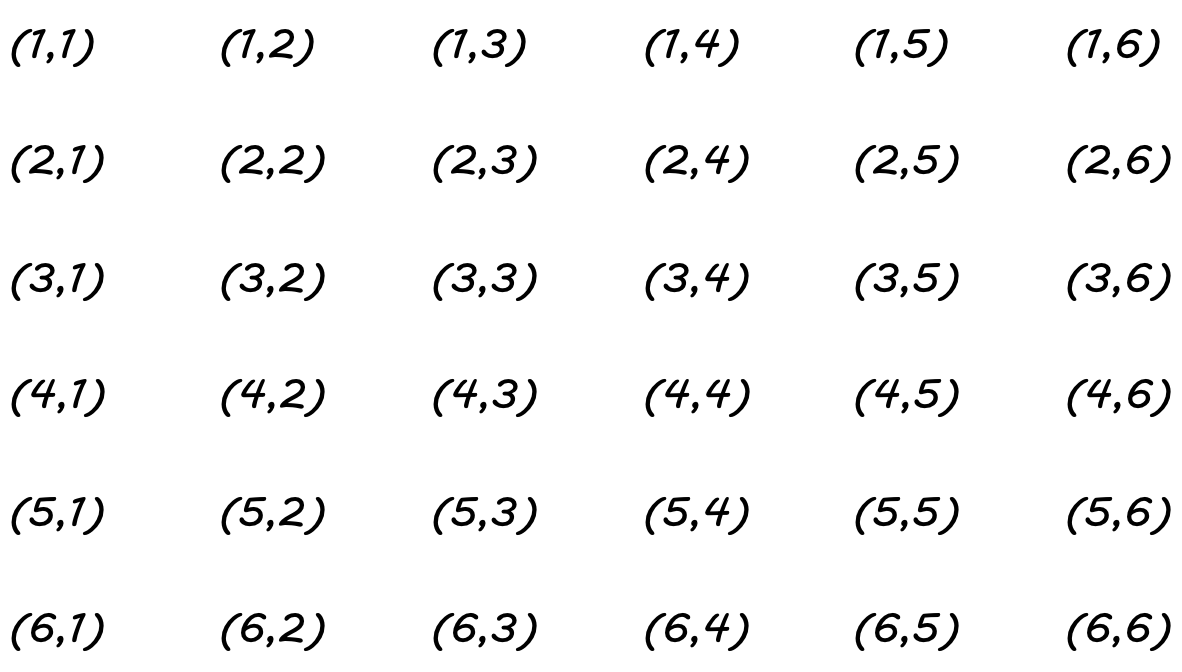
\includegraphics[scale=.3]{figs/SixesTable.png}

\vspace{1in}
\end{frame}



\begin{frame}
	\frametitle{Example }
	\begin{center}
	
\qbx[4.5in]{applegreen!40}{ \Exmpl{applegreen}{} Consider the experiment in which we  measure (in hours) the lifetime of a transistor.
\\\HLTW{\text{Experiment:}  } (in hours) the lifetime of a transistor.
}
\vspace{.1in}
\pause
\qBrd[4.5in]{ceil!40}{
\HLTW{\text{Sample Space:}} The sample space consists of
all non-negative real numbers; that is,
 $\SampleS=\HLTY{ \{x\in \R: x>0   \}}=\HLTY{\R_{+}}.$
}
\\
\pause
\vspace{.1in}
\qBrd[4.5in]{apricot!70}{ \Qn Let $\HLTY{A}$ be 
the event that  the transistor does not last longer than 5 hours.  Write down the event A in the notation of set theory.  }


\end{center}
\vspace{2.5in}

\end{frame}




\TransitionFrame[antiquefuchsia]{\Large Reminder:  Disjoint Events and Partition }




%
%\begin{frame}\frametitle{ Disjoint Events \& Partition}
%\begin{center}
%\vspace{-.7in}
%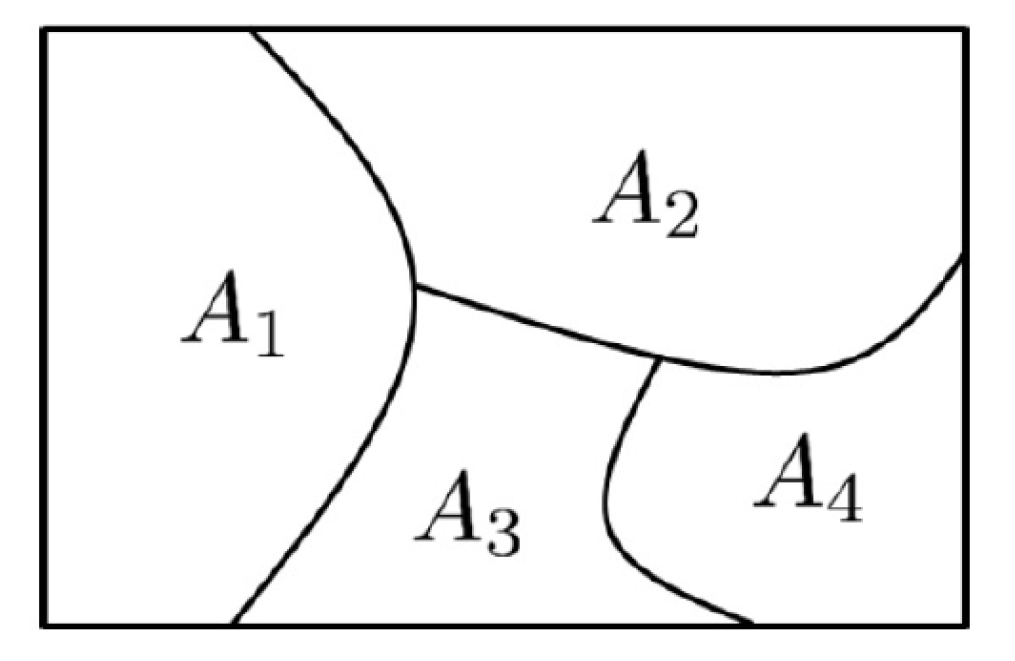
\includegraphics[scale=.4]{figs/VDPartition_0.png} 
%\end{center}
%\end{frame}


{
%\setbeamercolor{structure}{fg=antiquefuchsia!80, bg= black!60}
\setbeamercolor{structure}{fg=gray!30, bg= black!60}


\begin{frame}
	\frametitle{Reminder from Unit1 Slides: Disjoint Sets}
	\vspace{-.1in}
	\begin{center}
\qbx[4.3in]{teal!30}{\qBrd[1in]{olive!30}{\bf Disjoint Sets:}  Two sets  A, and  B are said to be  {\bf Disjoint Sets} or {\bf mutually exclusive sets} if $A$ and $B$ does not have any elements in common.\\
}\\
\vspace{-.2in}
  \qbx[3in]{applegreen!50}{  
 A and B are Disjoint $\Leftrightarrow \HLTY{A\cap B=\emptyset}$.
  }
  
  	\end{center}
	\vspace{4in}
	\end{frame}
	

%
%
%\begin{frame}
%	\frametitle{Reminder from Unit1 Slides: Partition}
%	\begin{center}
%\qbx[4.6in]{antiquebrass!60}{\qBrd[1in]{olive!30}{\bf Partition:}  A collection of sets $\HLTY{\{A_1, A_2, \cdots, A_k\}}$ is called a {\bf partition for a set $\HLTW{C}$} if
%\begin{enumerate}
%\item  \qBrd[3.5in]{applegreen!30}{$A_i \cap A_j = \emptyset$ for $1\leq i \neq j \leq k$ ({\tiny  i.e. ,$A_i$,  and $A_j$ are Disjoint if $i\neq j$}) }, and 
%\item  \qBrd[4in]{teal!30}{$\HLTY{A_1\cup A_2\cup \cdots \cup  A_k} =\HLTW{C}$.}
%\end{enumerate}
%}\\
%%\pause
%\vspace{.1in}
%  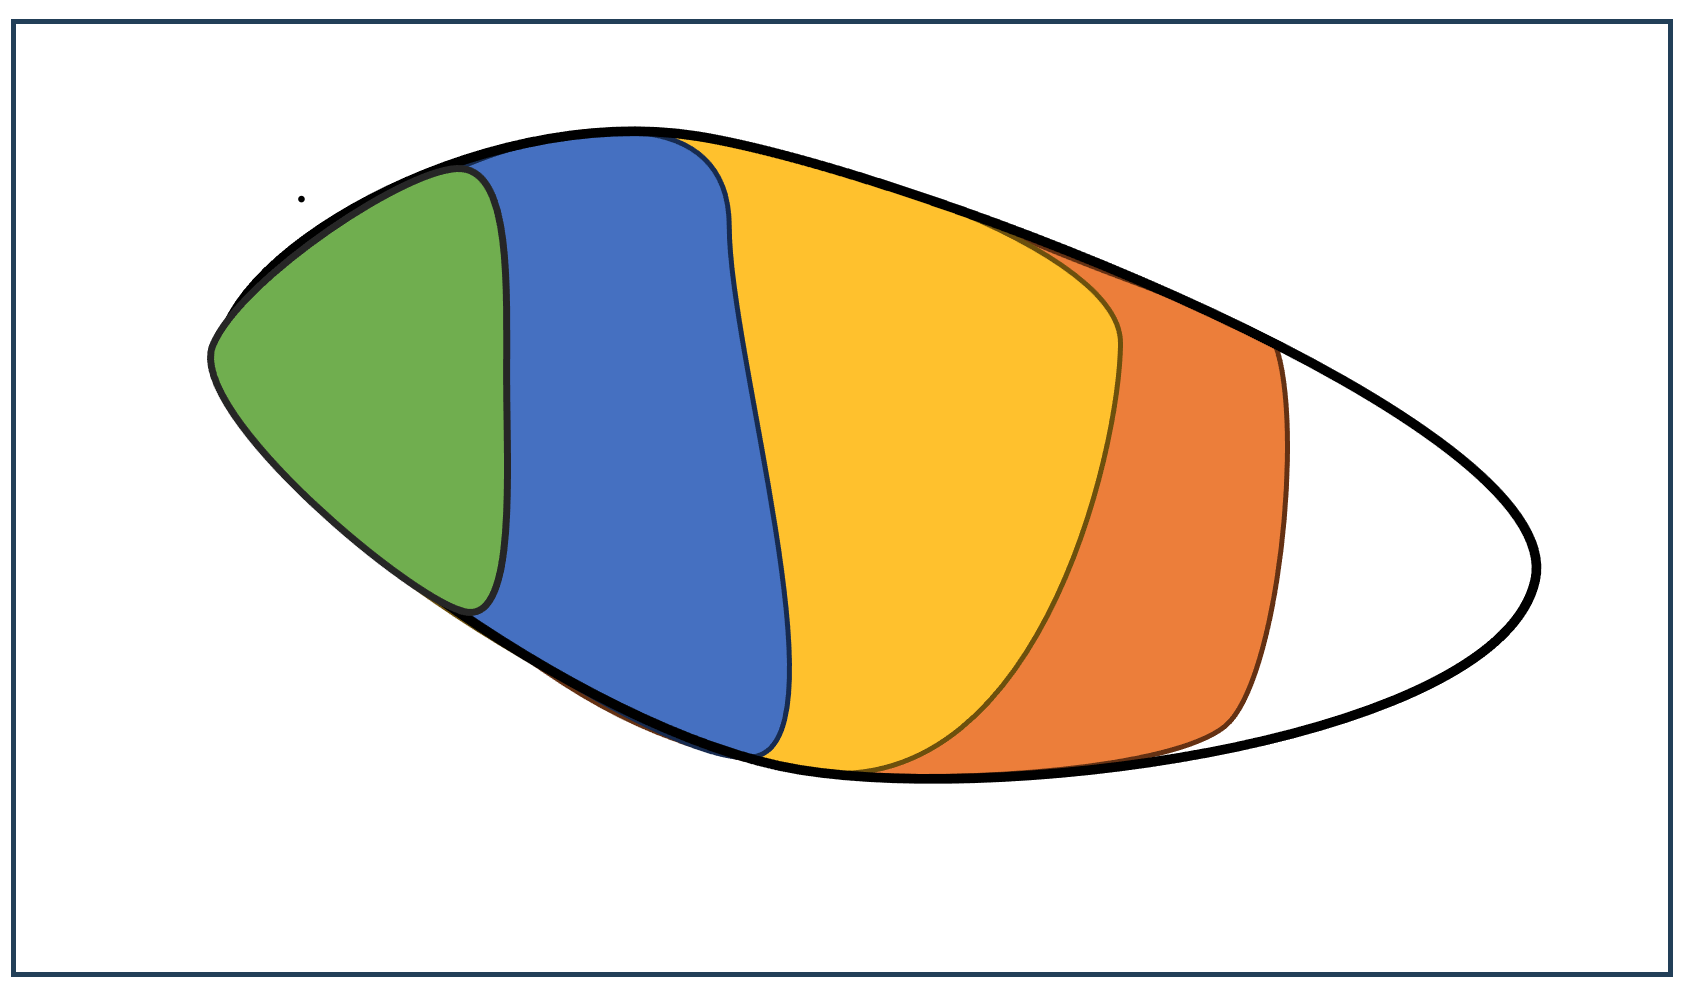
\includegraphics[scale=.2]{figs/VDPartition2.png} 
%  	\end{center}
%  	
%	\vspace{4in}
%	\end{frame}
%
%
%}

%
%\begin{frame}\frametitle{ Pairwise Disjoint Events }
%\vspace{-.1in}
%\begin{definition}[Pairwise Disjoint Events]
%A collection of events  $\{A_i\}_{i=1}^{k}$ are pairwise disjoint (or mutually exclusive) if $A_i \cap A_j=\emptyset$ for all $1\leq i \neq j\leq k$.
%\end{definition}
%\vspace{2in}
%\end{frame}







\begin{frame}\frametitle{ Pairwise Disjoint Events  }
\vspace{-.2in}
	\begin{center}
\qbx[4.6in]{amethyst!60}{\qBrd[1.9in]{olive!30}{\bf Pairwise Disjoint Events :}  A collection of sets $\HLTY{\{A_1, A_2, \cdots, A_k\}}$ are called  {\bf pairwise disjoint} events if \\
\qBrd[2.7in]{applegreen!30}{  $\HLTW{\HLTY{A_i \cap  A_j}= \emptyset} $ for all $i \neq j$.}
}\\
%\pause
%\vspace{.1in}
 % 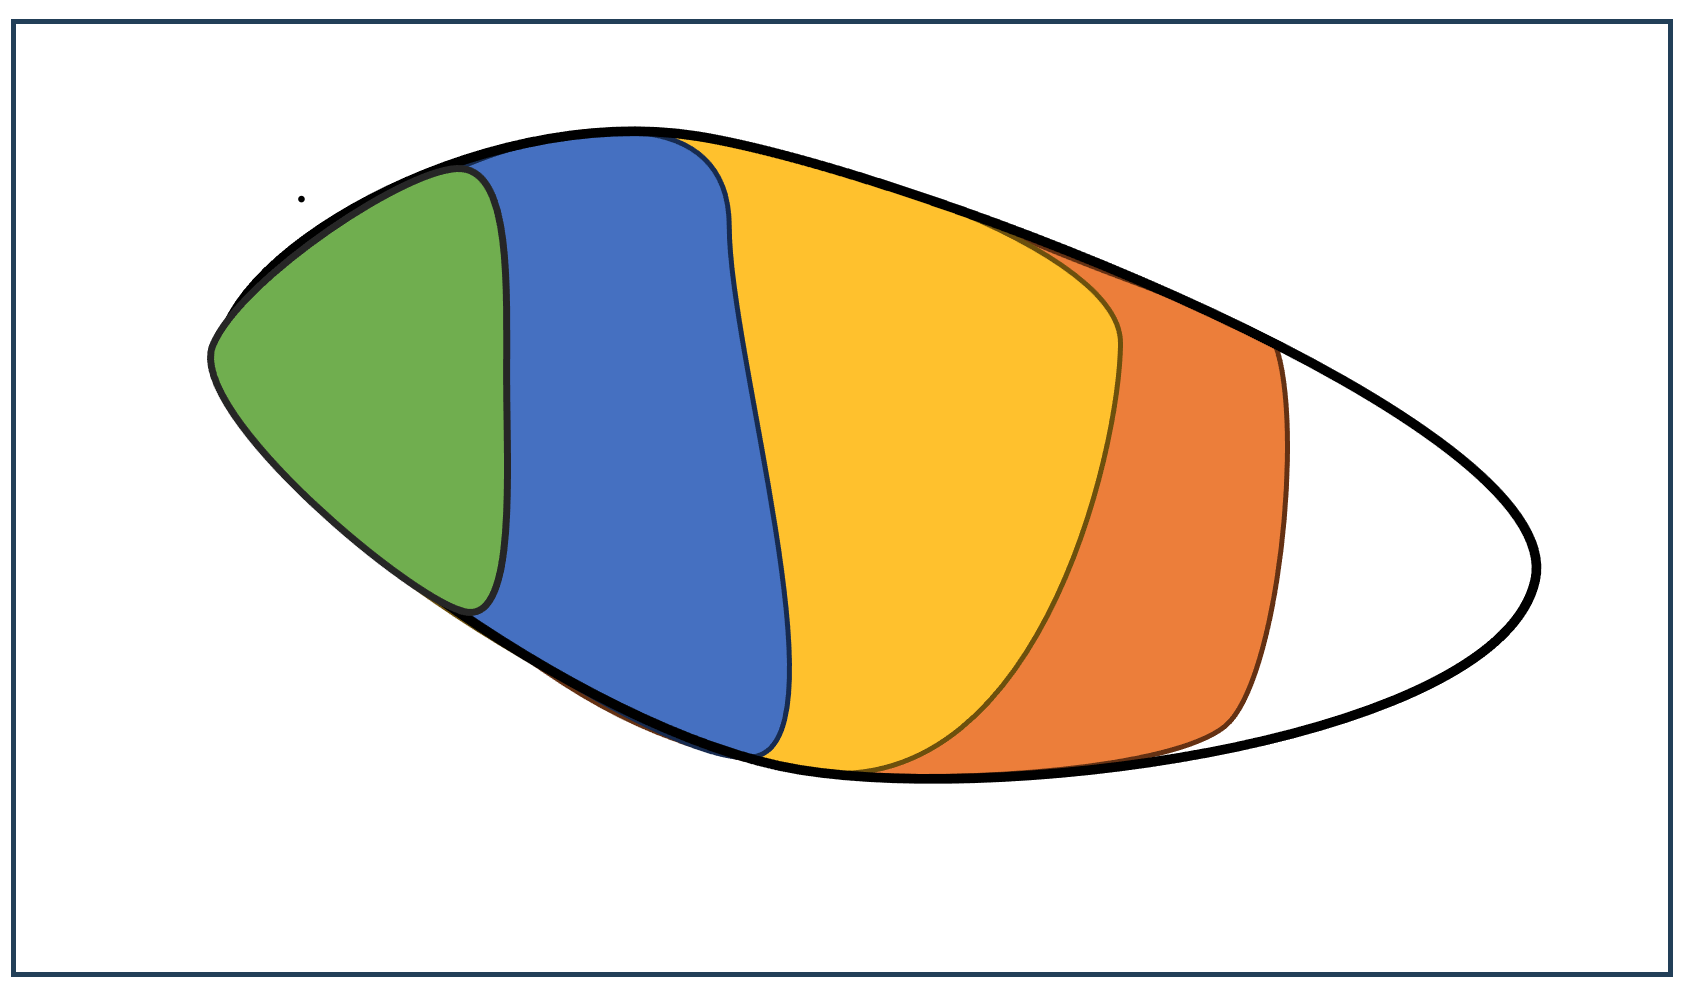
\includegraphics[scale=.2]{figs/VDPartition2.png} 
  	\end{center}
  	



\vspace{.1in}

\qBrd[4.5in]{bittersweet!50}{\HLTW{
Comment:}In the above definition, we may replace $\HLTY{n}$ by $\HLTY{\infty}$ and the definition extends naturally. }
%\pause
%\vspace{.1in}
%
%\qBrd[4.5in]{teal!50}{\HLTW{
%Comment:} Any set $\HLTY{A}$ and  it's complement,  $\HLTY{\Not{A}}$,  creates  a partition of $\HLTW{\SampleS}$.}


\end{frame}


}

%\define{Partition of Sample Space}{ $A_1,A_2, \ldots,  A_n$ are called partition of the sample space $\SampleS$ if $\{A_i\}_{i=1}^{n}$ is pairwise disjoint and $\HLTY{ \displaystyle \bigcup_{i=1}^{n} A_i=\SampleS.}$}
%\pause
%
%\begin{frame}\frametitle{  Partition of Sample Space}
%\vspace{-.2in}
%	\begin{center}
%\qbx[4.6in]{amethyst!60}{\qBrd[1.9in]{olive!30}{\bf Partition of Sample Space:}  A collection of sets $\HLTY{\{A_1, A_2, \cdots, A_n\}}$ is called a {\bf partition } for a set $\HLTW{\SampleS}$ if
%\begin{enumerate}
%  \item\qBrd[3.7in]{applegreen!30}{  the collection of events  $\HLTY{\{A_i\}_{i=1}^{n}}$ are {\bf pairwise disjoint} }
% , and 
% \item \qBrd[2.5in]{teal!30}{ $\HLTY{A_1\cup A_2\cup \cdots \cup  A_n} =\HLTW{\SampleS}$.}
%\end{enumerate}
%}\\
%%\pause
%%\vspace{.1in}
% % 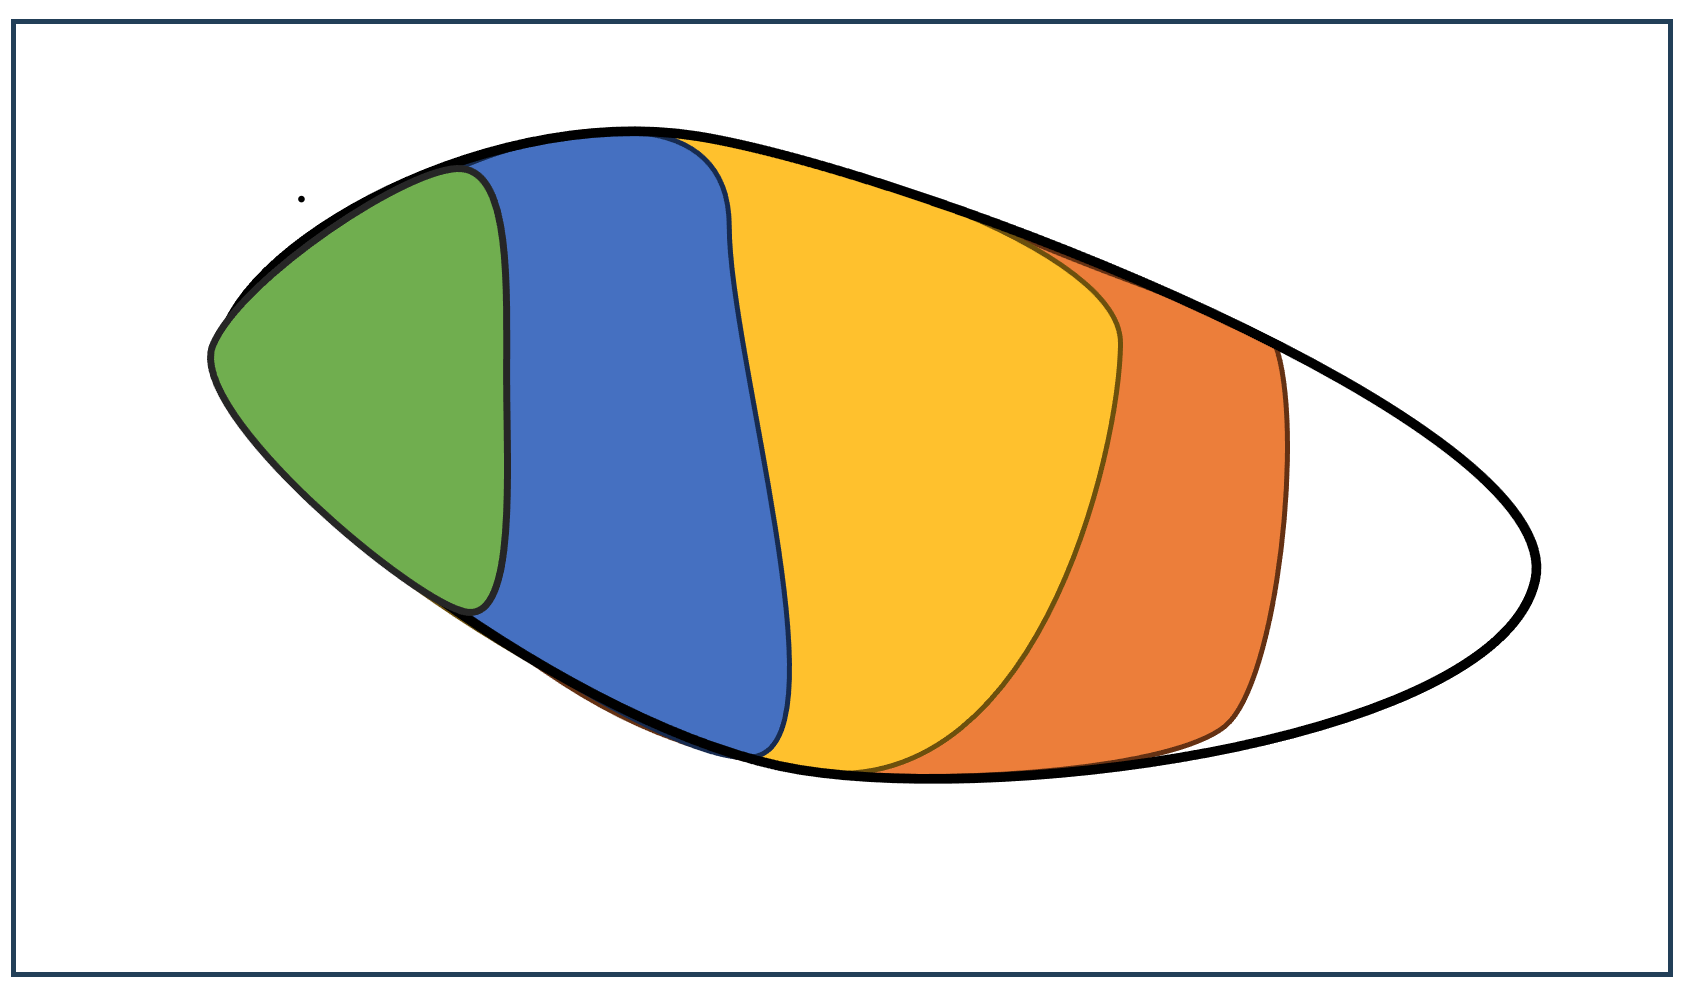
\includegraphics[scale=.2]{figs/VDPartition2.png} 
%  	\end{center}
%  	
%
%
%
%\vspace{.1in}
%
%\qBrd[4.5in]{bittersweet!50}{\HLTW{
%Comment:}In the above definition, we may replace $\HLTY{n}$ by $\HLTY{\infty}$ and the definition extends naturally. }
%\pause
%\vspace{.1in}
%
%\qBrd[4.5in]{teal!50}{\HLTW{
%Comment:} Any set $\HLTY{A}$ and  it's complement,  $\HLTY{\Not{A}}$,  creates  a partition of $\HLTW{\SampleS}$.}
%
%
%\end{frame}
%






\section{ The Notion of Probability}
\TransitionFrame[bittersweet]{\Large  Notion of Probability  }


\begin{frame}\frametitle{Basic Notion of Probability}
\begin{itemize}
\item {\bf Probability} refers to the chance that a particular event will
occur.
\vspace{.1in}
\item The probability of an event is the proportion of times the
event is expected to occur in repeated experiments.
\vspace{.1in}
\item If we denote by $\HLT[applegreen!40]{n(E)}$ the number of times in the first $\HLTY{n}$
repetitions of the experiment that the event $E$ occurs, the
probability of the event $E$ is defined by $$ \DBX{ \displaystyle P(E) =\lim_{n\mapsto\infty}
\frac{\HLT[applegreen!40]{n(E)}}{\HLTY{n}}.}$$
\end{itemize}
\end{frame}



\begin{frame}\frametitle{Axiomatic Definition of Probability}

\define{Probability}{
Consider an experiment whose sample space is $\SampleS$.  A  set-function $P(E)$,  defined for each event $E$ of $\SampleS$, is said to be a {\bf probability} if,   it satisfies the following three axioms
\begin{enumerate}
\qBrd[2.3in]{olive!30}{\item $\HLTW{0\leq P(E)\leq 1}$ for any event $E$}\\

\qBrd[2.7in]{babyblueeyes!50}{\item$\HLTW{ P(\SampleS)= 1}$}\\

\qBrd[4.2in]{ube!40}{\item For any sequence of mutually disjoint (mutually exclusive) events $E_1, E_2, E_3, \ldots ,  $ ({\tiny that is, events for which $E_i \cap E_j= \emptyset$ for all $i\neq j$})
\begin{center}
\qBrd[1.8in]{amethyst!70}{
$ \HLTW{ \displaystyle P\left(\bigcup_{i=1}^{\infty}E_i \right) = \sum_{i=1}^{\infty}P\left(E_i \right) }  $}\end{center}
}
\end{enumerate}
We refer to $P(E)$ as the {\bf probability} of the event $ E$.
}
\vspace{1.5in}

\end{frame}


\begin{frame}
\qbx[4.6in]{teal!40}{
\vspace{.2in}
\HLTW{Comment: } \\
\vspace{.05in}\\
\qBrd[4.4in]{applegreen!40}{{\bf Axiom 1} states that the probability of an event \HLTY{E} is always  between 0 and 1. }\\
\vspace{.05in}\\
\qBrd[4.4in]{olive!40}{{\bf Axiom 2} Probability of the entire sample space $\HLTW{\SampleS}$ is 1. }\\
\vspace{.05in}\\
\qBrd[4.4in]{lime!40}{{\bf Axiom 3} states that, for any sequence
of {\bf mutually exclusive events (i.e. disjoint events)}, the probability of at least one of these
events occurring is just the sum of their respective probabilities.
}
\vspace{.2in}
}
\end{frame}

\section{ A Few Properties of Probability}







%
%\begin{frame}{A Few Properties of Probability}
%Let $(\SampleS , P )$ be a sample space along with the Probability measure. Let $A, B$ are two events.  Then 
%\begin{itemize}
%\item 
%\item 
%\item
%\item If $A\subset B $ then $P(A)\leq P(B) $.
%\item
%\end{itemize}
%
%\vspace{2in}
%
%\end{frame}


\TransitionFrame[amethyst]{\Large A Few Properties of Probability  }

\begin{frame}\frametitle{  $P(\emptyset)= 0$, and   $P(\SampleS)= 1$}
\begin{center}

\includegraphics[scale=.45]{figs/SampleSpace.png} 
\end{center}
\vspace{1in}
\end{frame}


\begin{frame}\frametitle{  $P(A)\leq 1$}
\begin{center}
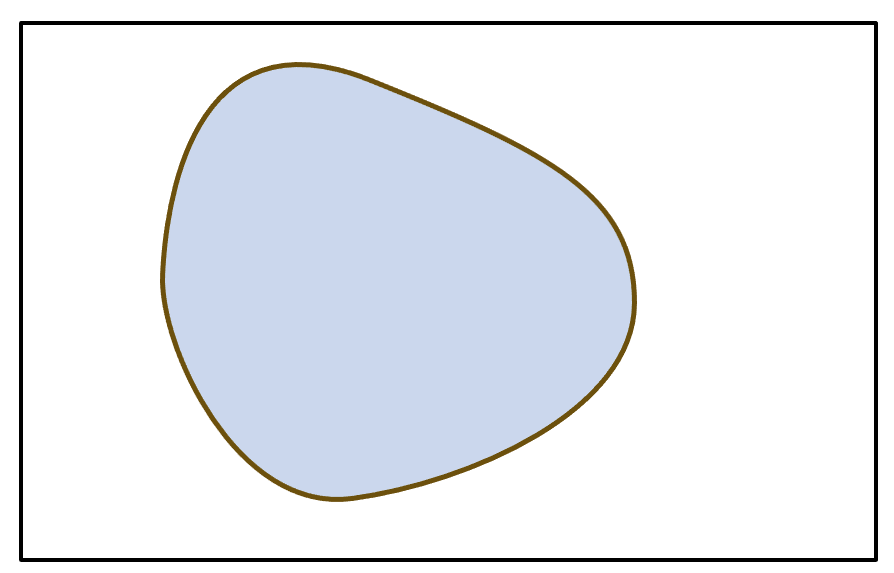
\includegraphics[scale=.4]{figs/PALess1.png} 
\end{center}
\vspace{1in}
\end{frame}



\begin{frame}\frametitle{ If $A\subset B $ then $P(A)\leq P(B) $}
\begin{center}
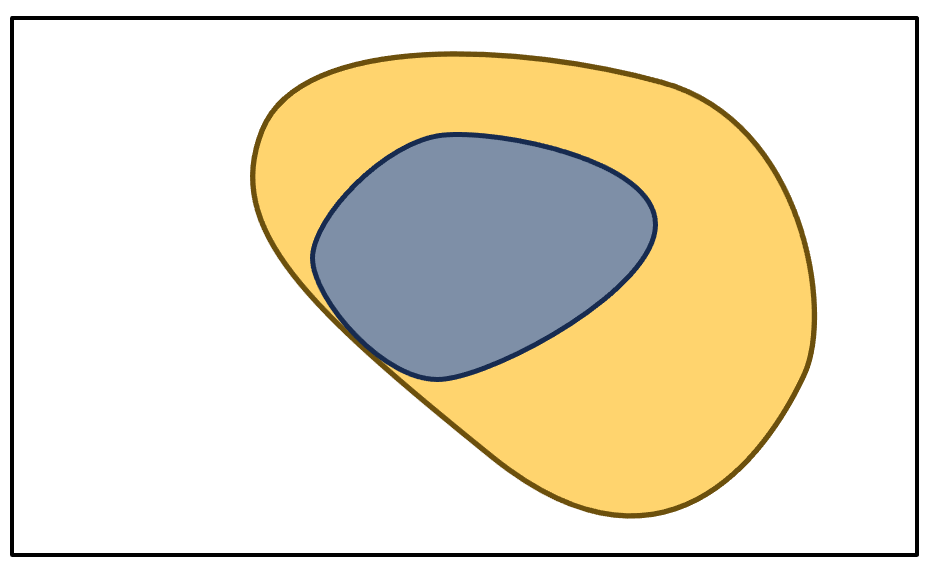
\includegraphics[scale=.4]{figs/PALessPB.png} 
\end{center}
\vspace{1in}
\end{frame}



\begin{frame}\frametitle{$P(\Not{A})=1-P(A)$}
\begin{center}
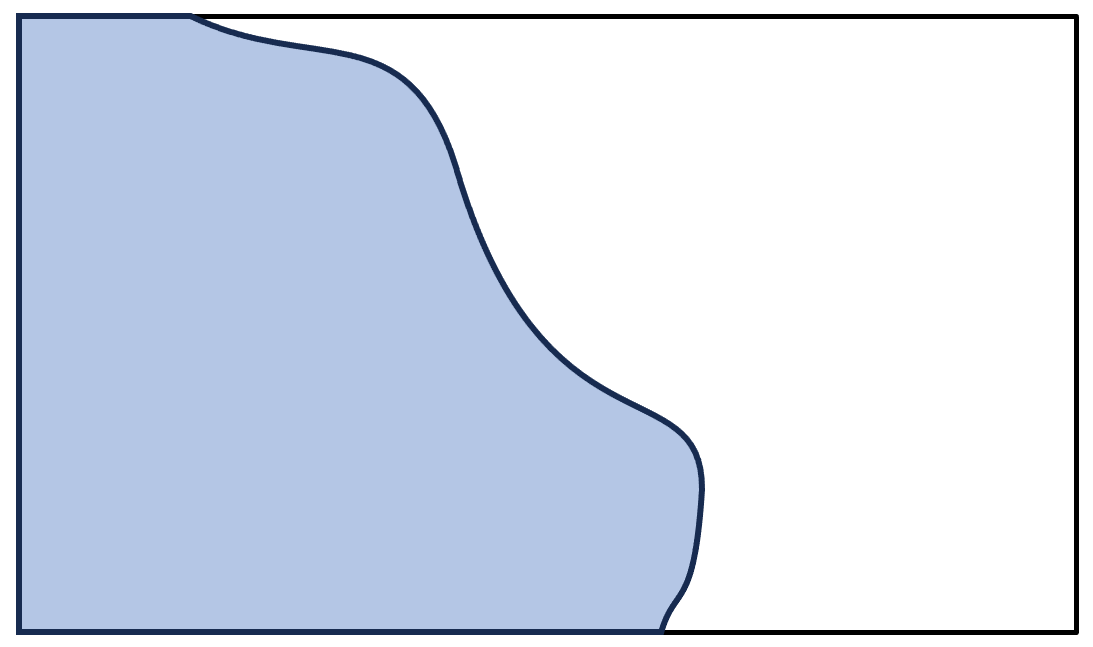
\includegraphics[scale=.26]{figs/A_complement.png} 
\end{center}
\vspace{1in}
\end{frame}


\begin{frame}\frametitle{$P(A\cup B)= P(A)+P(B)-P(A\cap B)$}
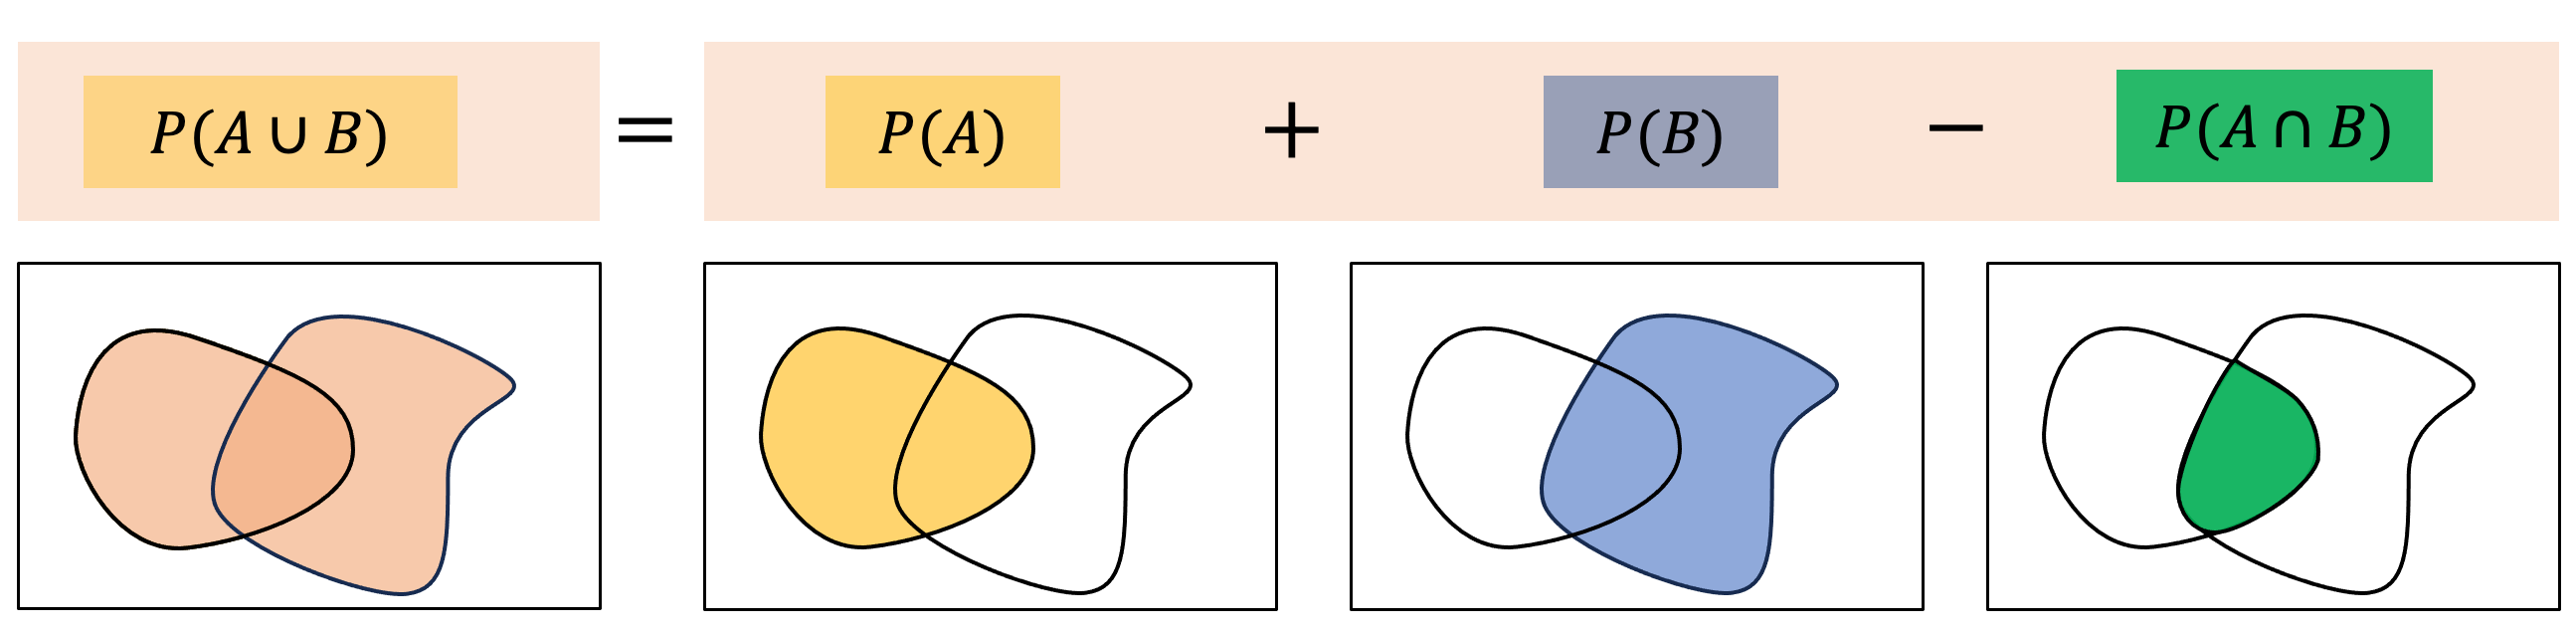
\includegraphics[scale=.26]{figs/P_A_UNION_B.png} 
\vspace{1in}
\end{frame}


\begin{frame}\frametitle{{Summary: A Few Properties of Probability}}
\qbx[4.6in]{antiquefuchsia!60}{
\vspace{.1in}
Let $\HLTY{(\SampleS , P)}$ be a sample space along with the Probability measure. Let $\HLTW{A}, \HLTW{B}$ be two events.  Then, \\
\begin{enumerate}
\qBrd[3.5in]{applegreen!40}{  \item[{\sqBullet{olive}}] $\HLTW{P(\emptyset)=0}$ where $\HLTW{\emptyset}$ denotes the Null set. }\\
\vspace{.05in}
\qBrd[2in]{apricot!40}{ \item[{\sqBullet{apricot}}]  $\HLTW{P(A)\leq 1}$. }\\
\vspace{.05in}
\qBrd[2.8in]{lime!40}{ \item[{\sqBullet{lime}}] If $\HLTW{
A\subseteq B}$ then $\HLTW{P(A)\leq P(B)} $.}\\
\vspace{.05in}
\qBrd[3.8in]{brightlavender!40}{\item[{\sqBullet{amethyst}}] $\HLTW{P(\Not{A})=1-P(A)}$, where  $\HLTW{\Not{A}}$ denotes the complementary event to $A$}\\
\vspace{.05in}
\qBrd[4in]{cadmiumorange!40}{\item[{\sqBullet{cadmiumorange}}]  $ \HLTW{P(A\cup B)= P(A)+P(B)-P(A\cap B) }$.}
\end{enumerate}
}
\end{frame}


\begin{frame}
\vspace{-.05in}
\qBox{ \Qn Represent the probability of the following events using $P(A), P(B)$ and $P(A\cap B)$. 
\begin{enumerate}
\item $P(A- B)= P(A\cap \Not{B})=?$
\item $P(B- A)=?$
\item If $A, B$ are disjoint, i.e. $A\cap B=\emptyset$ then what is $P(A\cup B) = ?$
\end{enumerate}
 }
% \pause 
 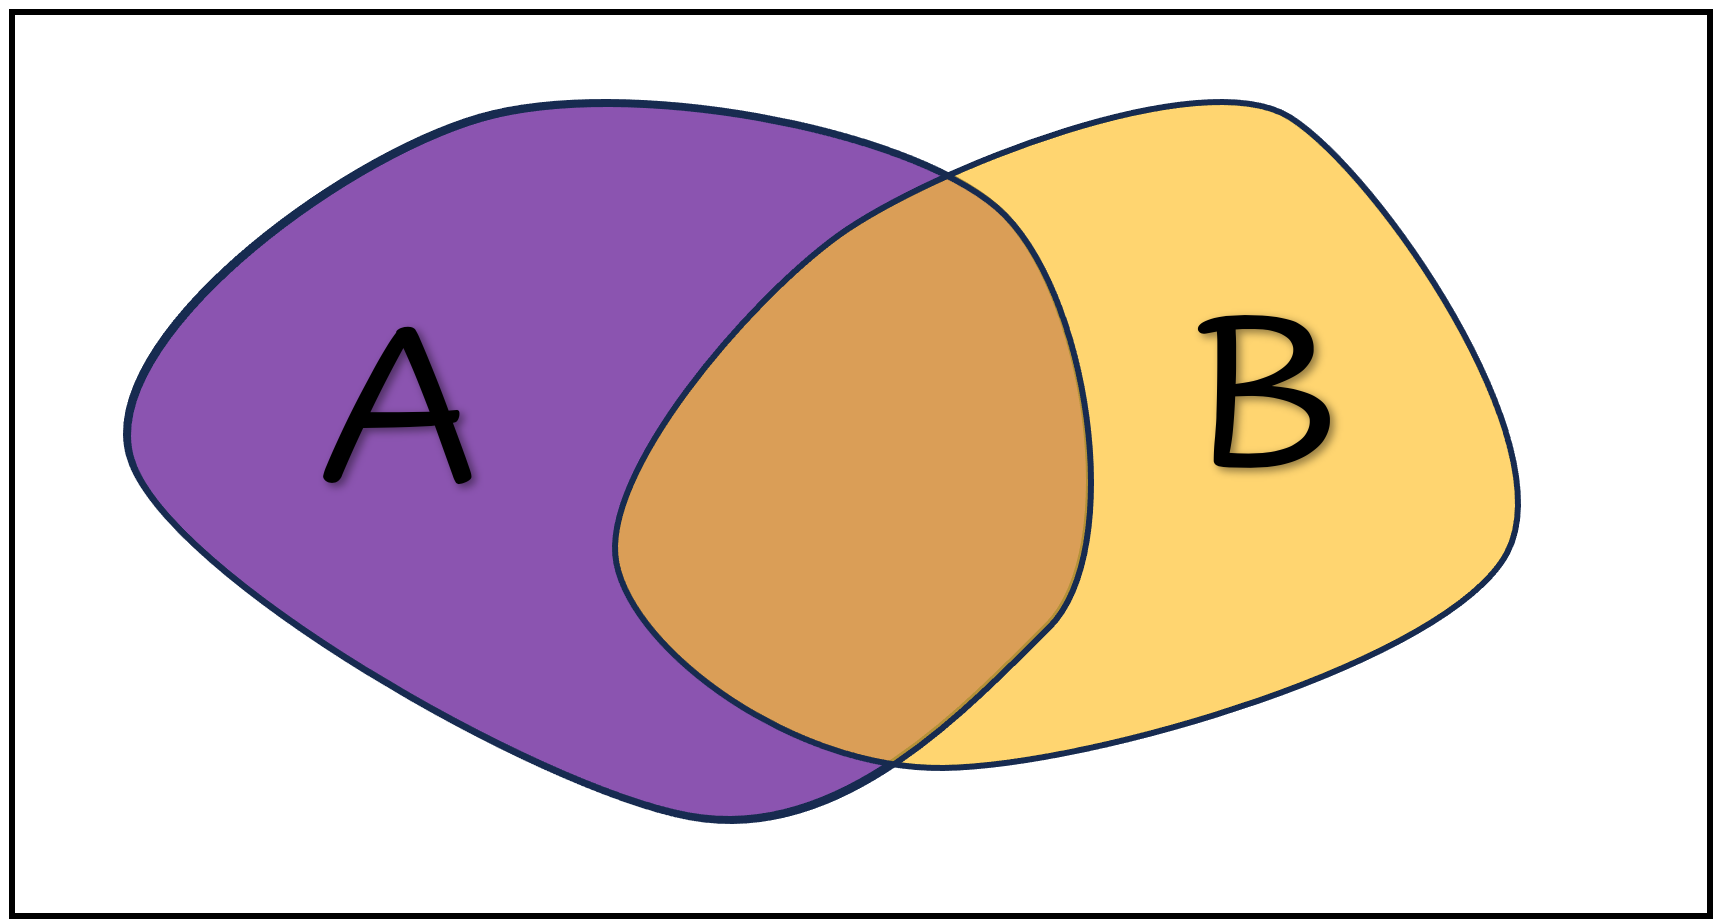
\includegraphics[scale=.18]{figs/AUB.png}
  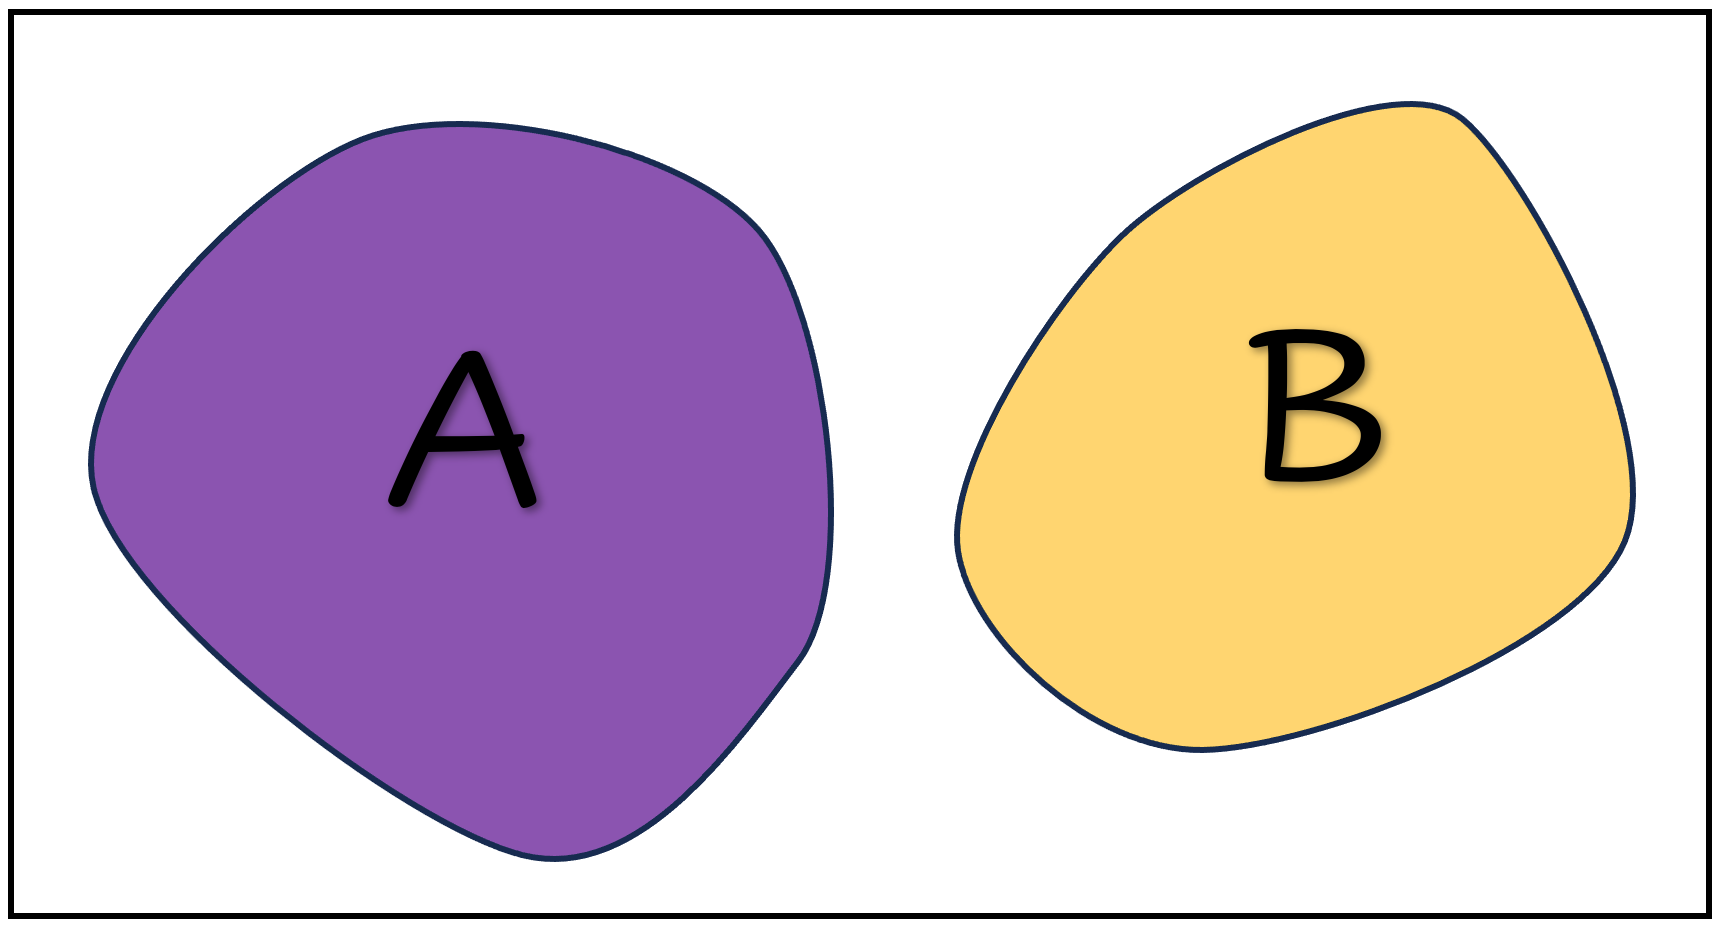
\includegraphics[scale=.18]{figs/AUB_Disjoint.png}
 \vspace{2in}
 
\end{frame}





\begin{frame}{ Examples}
\vspace{-.1in}
\qbx[4.5in]{bronze!40}{
\Exmpl{bronze}{} \small A smoke detector system uses two devices, A and B. If smoke is present, the probability that
it will be detected by device \HLTY{A} is \HLTW{0.95}; by device \HLTY{B},\HLTW{0.90}; and by both devices, \HLTW{0.88}.
\begin{enumerate}
\item If smoke is present, find the probability that the smoke will be \HLTW{\text{detected by either device A or B, or both devices.}}
\item Find the probability that the smoke will be undetected.
\end{enumerate}
 }

\vspace{.5in}
\pause
{\tiny
Solution: A: \{device A detects smoke\}   B: \{device B detects smoke\}

$P(A\cup B)= P(A)+P(B)=P(A\cap B)= 0.95+0.90-0.88=.97$

$P(\text{Smoke is undetected })=1- P(\text{Smoke is detected by atleast one devices })  =  1-P(A\cap B)=1-0.97=0.03$

}

%{\tiny
%Solution: A: \{device A detects smoke\}   B: \{device B detects smoke\}
%
%$P(A\cup B)= P(A)+P(B)=P(A\cap B)= 0.95+0.90-0.88=.97$
%
%$P(\text{Smoke is undetected })=1- P(\text{Smoke is detected by atleast one devices })  =  1-P(A\cap B)=1-0.97=0.03$
%
%}

\end{frame}









\begin{frame}{ Examples}
\vspace{-.1in}
\qbx[4.5in]{babyblue!40}{
\Exmpl{babyblue!50}{} Suppose that A and B are mutually exclusive events for which \HLTW{P(A) =0 .3} and \HLTW{P(B) = 0.5}. What is the probability that 
\vspace{-.1in}
\begin{enumerate}
\item either A or B occurs?
\item A occurs but B does not?
\item both A and B occur?
\end{enumerate}
 }

\vspace{1in}


\end{frame}


\begin{frame}\frametitle{A Standard Prototype: Two Cross Two Table}
\begin{center}
\qBrd[4.6in]{babyblue!30}{
\begin{center}
\begin{tabular}{|l||l|l||l|l|}
\hline
      & $A$ & $\Not{A}$ & Marginal of $B$   \\ \hline\hline
$B$ &  $\HLTEQ[olive!30]{P(A\cap B)}$   &    $\HLTY{P(\Not{A}\cap B)}$ &  $\HLTW{P(B)}$    \\ \hline
$\Not{B}$ &   $\HLTY{P(A\cap \Not{B})}$  &  $\HLTEQ[amethyst!40]{P(\Not{A}\cap \Not{B})}$   &   $\HLTW{P(\Not{B})}$    \\ \hline\hline
Marginal of $A$ & $\HLTW{P(A)}$     & $\HLTW{P(\Not{A})}$     &$ \HLTW{\text{Total Probability}= \HLTEQ[teal!40]{1}} $   \\ \hline
\end{tabular}
\end{center}
}
\end{center}
\vspace{1in}


\end{frame}




\begin{frame}{ Examples}
\vspace{-.1in}
\qbx[4.5in]{babyblue!40}{\small
\Exmpl{babyblue!50}{} Suppose that A and B are mutually exclusive events for which \HLTW{P(A) =0 .3} and \HLTW{P(B) = 0.5}. What is the probability that 
\vspace{-.1in}
\begin{enumerate}
\item either A or B occurs?
\item A occurs but B does not?
\item both A and B occur?
\end{enumerate}
 }
 
 \pause
 \vspace{.4in}
 \begin{center}
\qBrd[4.6in]{babyblue!30}{
\begin{center}
\begin{tabular}{|l||l|l||l|l|}
\hline
      & $A$ & $\Not{A}$ & Marginal of $B$   \\ \hline\hline
$B$ &  $\HLTEQ[olive!30]{\color{olive!30}P(A\cap B)}$   &    $\HLTY{\color{yellow}P(\Not{A}\cap B)}$ &  $\HLTW{\color{white}P(B)}$    \\ \hline
$\Not{B}$ &   $\HLTY{\color{yellow} P(A\cap \Not{B})}$  &  $\HLTEQ[amethyst!40]{\color{amethyst!40} P(\Not{A}\cap \Not{B})}$   &   $\HLTW{\color{white}P(\Not{B})}$    \\ \hline\hline
Marginal of $A$ & $\HLTW{\color{white}P(A)}$     & $\HLTW{\color{white} P(\Not{A})}$     &$ \HLTW{\text{Total Probability}= \HLTEQ[teal!40]{\color{teal!40}1}} $   \\ \hline
\end{tabular}
\end{center}
}
\end{center}

\vspace{1in}


\end{frame}




\begin{frame}{ Examples}
\vspace{-.1in}
\qbx[4.5in]{bronze!40}{ \small
\Exmpl{bronze}{} \small A smoke detector system uses two devices, A and B. If smoke is present, the probability that
it will be detected by device \HLTY{A} is \HLTW{0.95}; by device \HLTY{B},\HLTW{0.90}; and by both devices, \HLTW{0.88}.
\begin{enumerate}
\item If smoke is present, find the probability that the smoke will be \HLTW{\text{detected by either device A or B, or both devices.}}
\item Find the probability that the smoke will be undetected.
\end{enumerate}
 }

 \pause
\vspace{.1in}
 \begin{center}
\qBrd[4.6in]{babyblue!30}{
\begin{center}
\begin{tabular}{|l||l|l||l|l|}
\hline
      & $A$ & $\Not{A}$ & Marginal of $B$   \\ \hline\hline
$B$ &  $\HLTEQ[olive!30]{\color{olive!30}P(A\cap B)}$   &    $\HLTY{\color{yellow}P(\Not{A}\cap B)}$ &  $\HLTW{\color{white}P(B)}$    \\ \hline
$\Not{B}$ &   $\HLTY{\color{yellow} P(A\cap \Not{B})}$  &  $\HLTEQ[amethyst!40]{\color{amethyst!40} P(\Not{A}\cap \Not{B})}$   &   $\HLTW{\color{white}P(\Not{B})}$    \\ \hline\hline
Marginal of $A$ & $\HLTW{\color{white}P(A)}$     & $\HLTW{\color{white} P(\Not{A})}$     &$ \HLTW{\text{Total Probability}= \HLTEQ[teal!40]{\color{teal!40}1}} $   \\ \hline
\end{tabular}
\end{center}
}
\end{center}

\end{frame}








\begin{frame}

\qbx[4.5in]{olive!40}{
\Exmpl{olive}{}  An evaluation of a small business by an accounting firm either reveals a problem with the accounts or it doesn't reveal a problem.  Also, the evaluation is either done
accurately or incorrectly. The probability that the
evaluation is done accurately is 0.85. Furthermore, the
probability that the evaluation is done incorrectly and that
it reveals a problem is 0.10. If the probability that the
evaluation is done accurately and it does not reveal a
problem is 0.25, what is the probability that the
evaluation does not reveal a problem?
 }


%\pause
 \pause
%\vspace{.05in}
 \begin{center}
\qBrd[4.6in]{babyblue!30}{
\begin{center}
\begin{tabular}{|l||l|l||l|l|}
\hline
      & $A$ & $\Not{A}$ & Marginal of $B$   \\ \hline\hline
$B$ &  $\HLTEQ[olive!30]{\color{olive!30}P(A\cap B)}$   &    $\HLTY{\color{yellow}P(\Not{A}\cap B)}$ &  $\HLTW{\color{white}P(B)}$    \\ \hline
$\Not{B}$ &   $\HLTY{\color{yellow} P(A\cap \Not{B})}$  &  $\HLTEQ[amethyst!40]{\color{amethyst!40} P(\Not{A}\cap \Not{B})}$   &   $\HLTW{\color{white}P(\Not{B})}$    \\ \hline\hline
Marginal of $A$ & $\HLTW{\color{white}P(A)}$     & $\HLTW{\color{white} P(\Not{A})}$     &$ \HLTW{\text{Total Probability}= \HLTEQ[teal!40]{\color{teal!40}1}} $   \\ \hline
\end{tabular}
\end{center}
}
\end{center}
\end{frame}



\begin{frame}{ Examples}
\vspace{-.2in}
\qbx[4.55in]{airforceblue!40}{
\Exmpl{airforceblue}{} A car repair can be performed either on time or late and either satisfactorily or unsatisfactorily. The probability
of a repair being on time and satisfactory is 0.26. The
probability of a repair being on time is 0.74. The
probability of a repair being satisfactory is 0.41. What is
the probability of a repair being late and unsatisfactory?
 }

 \pause
\vspace{.2in}
 \begin{center}
\qBrd[4.6in]{babyblue!30}{
\begin{center}
\begin{tabular}{|l||l|l||l|l|}
\hline
      & $A$ & $\Not{A}$ & Marginal of $B$   \\ \hline\hline
$B$ &  $\HLTEQ[olive!30]{\color{olive!30}P(A\cap B)}$   &    $\HLTY{\color{yellow}P(\Not{A}\cap B)}$ &  $\HLTW{\color{white}P(B)}$    \\ \hline
$\Not{B}$ &   $\HLTY{\color{yellow} P(A\cap \Not{B})}$  &  $\HLTEQ[amethyst!40]{\color{amethyst!40} P(\Not{A}\cap \Not{B})}$   &   $\HLTW{\color{white}P(\Not{B})}$    \\ \hline\hline
Marginal of $A$ & $\HLTW{\color{white}P(A)}$     & $\HLTW{\color{white} P(\Not{A})}$     &$ \HLTW{\text{Total Probability}= \HLTEQ[teal!40]{\color{teal!40}1}} $   \\ \hline
\end{tabular}
\end{center}
}
\end{center}
\end{frame}




\begin{frame}

 
 \qBox{\Qn
Let $A, B$ be two events such that  $$P(A) = \frac{1}{3} \text{ and } P(\Not{B}) = \frac{1}{4}.$$Can A and B be disjoint? Explain.}
 \vspace{2in}
\end{frame}






%
%\begin{frame}{ Examples}
%
%\qbx[4.5in]{antiquefuchsia!40}{
%\Exmpl{antiquefuchsia}{}  In a study of patients arriving at a hospital emergency room, the gender of the patients is considered, together
%with whether the patients are younger or older than
%30 years of age, and whether or not the patients are
%admitted to the hospital. It is found that 45\% of the
%patients are male, 30\% of the patients are younger than
%30 years of age, 15\% of the patients are females older
%than 30 years of age who are admitted to the hospital, and
%21\% of the patients are females younger than 30 years of
%age. What proportion of the patients are females older
%than 30 years of age who are not admitted to the hospital?
% }
%
%\vspace{1in}
%%\pause
%{\tiny
%Solution: % A. 0.10 B. 0.20 C. 0.30 D. 0.40
%}
%\end{frame}
%
%\begin{frame}
% \pause
%\vspace{.1in}
% \begin{center}
%\qBrd[4.6in]{babyblue!30}{
%\begin{center}
%\begin{tabular}{|l||l|l||l|l|}
%\hline
%      & $A$ & $\Not{A}$ & Marginal of $B$   \\ \hline\hline
%$B$ &  $\HLTEQ[olive!30]{\color{olive!30}P(A\cap B)}$   &    $\HLTY{\color{yellow}P(\Not{A}\cap B)}$ &  $\HLTW{\color{white}P(B)}$    \\ \hline
%$\Not{B}$ &   $\HLTY{\color{yellow} P(A\cap \Not{B})}$  &  $\HLTEQ[amethyst!40]{\color{amethyst!40} P(\Not{A}\cap \Not{B})}$   &   $\HLTW{\color{white}P(\Not{B})}$    \\ \hline\hline
%Marginal of $A$ & $\HLTW{\color{white}P(A)}$     & $\HLTW{\color{white} P(\Not{A})}$     &$ \HLTW{\text{Total Probability}= \HLTEQ[teal!40]{\color{teal!40}1}} $   \\ \hline
%\end{tabular}
%\end{center}
%}
%\end{center}
%\end{frame}
%
%



\TransitionFrame[bittersweet]{\Large Inclusion Exclusion Principle  }


%__________________________________________
\begin{frame}{Inclusion Exclusion Principle: Specific Case  $n=3$}
\qBox{
Let $A_1, A_2, A_3$ are three events.  Then 
\begin{eqnarray*}
 P\left(A_1\cup A_2 \cup A_3\right) 
 & =&  \left\{ \HLTEQ{P(A_1)+P(A_2)+P(A_3)}\right\}  \nonumber\\
 & &-  \left\{\HLTEQ[lightBlueOne]{ P(A_1\cap A_2) + P(A_1\cap A_3) + P(A_2\cap A_3) }  \right\}\\
 & & + \left\{ \HLTEQ{P(A_1\cap A_2 \cap A_3)}     \right\}  
\end{eqnarray*}  
}


\end{frame}
%__________________________________________
\begin{frame}{Inclusion Exclusion Principle}

\begin{lemma}
Let  $\{A_i\}_{i=1}^{n}$ be a sequence of events, for all $i=1, 2, 3, \ldots, n $. Then 
$$  P\left(\bigcup_{i=1}^{n}A_i \right)= \sum_{\HLTY{k}=1}^{n } \sum_{\HLTEQ[white]{\HLTEQ[lightBlueTwo]{(i_1,i_2,\ldots,{\HLTY{i_k}})\in \mathbb{Q}_{n,k}}}} (-1)^{\HLTY{k+1}}P\left(\bigcap_{m=1}^{k} A_{i_m} \right) ,  $$
where   $ \HLTEQ[white]{\HLTEQ[lightBlueTwo]{\mathbb{Q}_{n,k}:= \left\{(i_1, i_2\ldots, i_k)\in \mathbb{Z}_{+}^k: 1\leq i_1<i_2<\ldots<i_{k}\leq n \right\} }}.$ 
\end{lemma}
$\mathbb{Q}_{4, 2}=\left\{   \HLTEQ{(1, 2), (1, 3), (1, 4)},  \HLTEQ[lightBlueOne]{(2, 3), (2, 4)},  \HLTEQ[lightGreenTwo]{(3, 4)}   \right\},$
$\mathbb{Q}_{4, 3}=\left\{   \HLTEQ{(1, 2, 3), (1, 3, 4)},  \HLTEQ[lightGreenTwo]{(2, 3, 4)}\right\},$\\
$$\HLTEQ[lightBrownOne]{ \HLTEQ[white]{  \mathbb{Q}_{3, 1}=?,\mathbb{Q}_{3, 2}=?}}$$



\end{frame}


\section{Examples}



\TransitionFrame[antiquefuchsia]{\Large A Few Examples: \\
 assuming $ \HLTW{ \SampleS \text{ to be a finite set. }}$ }



\begin{frame}\frametitle{Finite Sample Spaces with Equally Likely Outcomes}

\qBrd[4.6in]{amethyst!40}{\sqBullet{amethyst} In many experiments, it is natural to assume that all outcomes in the sample space are equally likely to occur. }\\
\pause
\vspace{.15in}
\qBrd[4.6in]{olive!35}{\sqBullet{olive}  Consider the context when the sample space $\HLTW{\SampleS}$ is a finite set.  To be specific, let $\HLTW{\SampleS=\HLTY{\{1, 2, 3, \ldots, N\}}}.$ If we assume that all the outcome is equally likely,  then 
$\HLTW{P(\HLTY{\{1\}})=P(\HLTY{\{2\}})=\cdots =P(\HLTY{\{N\}})}$. 
It is intuitive and also easy to derive using Axioms 2 and Axiom3 of Probability that \\
\vspace{-.2in}
\begin{center}
\qBrd[2.5in]{teal!50}{$\HLTW{P(\HLTY{ \{i\}} )=\frac{1}{N}}$ for all $i=1,\ldots N$.}
\end{center} }
\vspace{.05in}
%\qBrd[4.7in]{babyblue!40}{\sqBullet{babyblue}  In equally-likely setup, it follows from Axiom 3 that, for any event $E$,  $$P(E)=\frac{\text{Number of outcomes in E}}{\text{Number of outcomes in }  \SampleS}.$$
%\vspace{-.2in}
%}
%\vspace{.05in}
%\qBrd[4.6in]{applegreen!40}{\sqBullet{applegreen}  In words, if we assume that all outcomes of an experiment are equally likely to occur, then the probability of any event $E$ equals the proportion of outcomes in the sample space that are contained in $E$.
%}
\end{frame}



\begin{frame}\frametitle{Finite Sample Spaces with Equally Likely Outcomes}

%\qBrd[4.6in]{amethyst!40}{\sqBullet{amethyst} In many experiments, it is natural to assume that all outcomes in the sample space are equally likely to occur. }\\
%\vspace{.05in}
%\qBrd[4.6in]{olive!40}{\sqBullet{olive}  That is, consider an experiment whose sample space $\SampleS$ is a finite set, say,  $\SampleS=\{1, 2, 3, \ldots, N\}.$ Then it is often natural to assume that  $P(\{1\})=P(\{2\})=\ldots =P(\{N\})$  which implies, from
%Axioms 2 and 3, that $P(\{i\})=\frac{1}{N}$ for all $i=1,\ldots N$. }\\
%\vspace{.05in}
\qBrd[4.5in]{ube!30}{\sqBullet{amethyst} If the sample space $\SampleS$ is finite and all the corresponding outcomes ( {\tiny elements in $\SampleS$})  are equally-likely,  then it follows from Axiom 3 that, for any event $E$,  
\vspace{-.12in}
\begin{center}
\qBrd[2.5in]{amethyst!60}{\;$\HLTW{\displaystyle P(E)=\frac{\text{Number of elements in E}}{\text{Number of elements in }  \SampleS}}\;$}
\end{center}
\vspace{.05in}
}

\vspace{.3in}
\qBrd[4.5in]{applegreen!40}{\sqBullet{applegreen}  Assuming the finite sample space,  if all the outcomes are equally likely to occur, then the probability of any event $E$ equals the proportion of outcomes in the sample space that are contained in $E$.
}
\end{frame}





\begin{frame}
\begin{itemize}
\qBrd[4.2in]{amethyst!50}{
\item[\sqBullet{amethyst}] To refer to the $\HLTW{\text{``Equally Likely Setup''}}$ we typically use the phrases such as the $\HLTW{\text{``Fair Coin"}}$ or  $\HLTW{\text{``Fair Dice"}}$
}\\

\vspace{.5in}
\qBrd[4.2in]{olive!30}{
\item[\sqBullet{olive}] For problems with Dice and Coins, unless otherwise specified,  we assume it to be a $\HLTW{\text{``Fair Coin''}}$ or $\HLTW{\text{``Fair Dice"}}$.  }
\end{itemize}

\end{frame}









\begin{frame}\frametitle{Example}
\qbx[4.5in]{amethyst!40}{
\Exmpl{amethyst}{} Two fair-dice are rolled and the two numbers that appears are recorded.    Let $A$ be the event that the First roll results in a Six while $B$ represent the event that the second roll is a Six.  
\begin{enumerate}
\item What is $P(A)$, $P(B)$, and $P(A\cup B)$?
\item What is the probability that the sum of the upturned faces will equal 8?
\end{enumerate} 
}\\
\vspace{.1in}
\pause
\;\;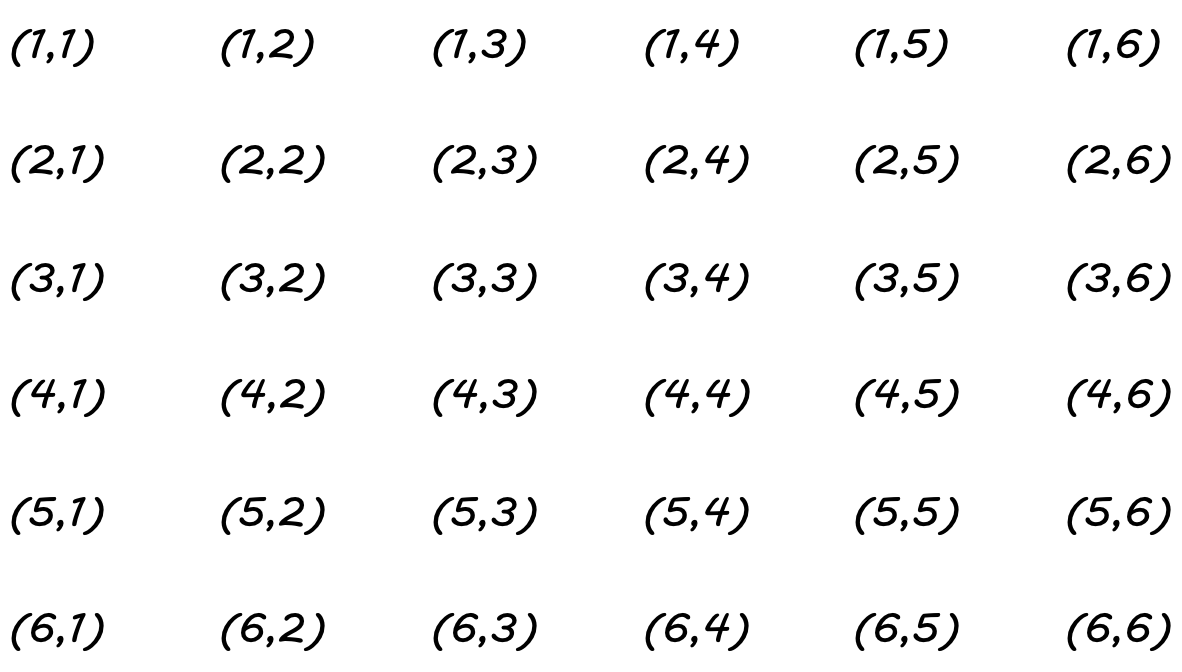
\includegraphics[scale=.26]{figs/SixesTable.png}\\
\vspace{1in}


\end{frame}

\begin{frame}\frametitle{Example}
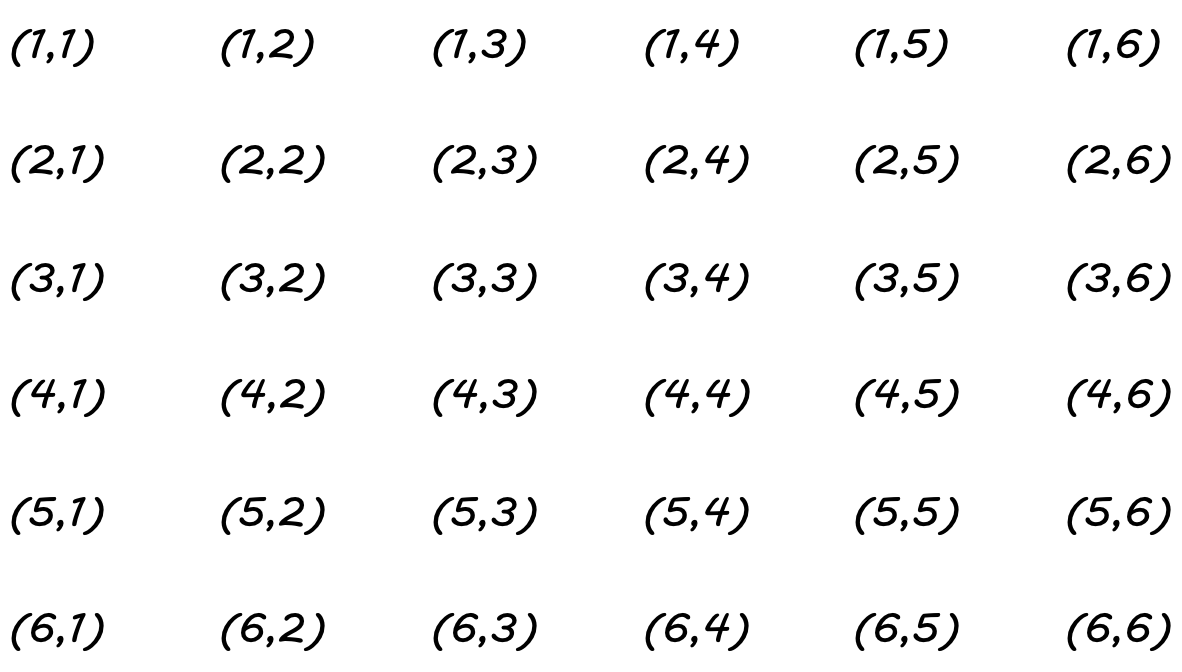
\includegraphics[scale=.3]{figs/SixesTable.png}\\
%\vspace{.5in}
\pause
\vspace{.2in}
{\tiny{ \bf Solution:} 
\qBrd[4.6in]{babyblue!30}{
1) $A=\{(6,1), (6,2), (6,3), (6,4), (6,5), (6,6)\}$, $P(A)=\frac{6}{36}=\frac{1}{36}$\\
$B=\{(1,6), (2,6), (3,6), (4,6), (5,6), (6,6)\}$, $P(B)=\frac{6}{36}=\frac{1}{36}$\\
$A\cap B= \{(6,6)\}$, $P(A\cap B)= \frac{1}{36}$\\
$P(A\cup B)= P(A)+P(B)-P(A\cap B)= \frac{1}{6}+  \frac{1}{6}- \frac{1}{36}= \frac{11}{36}$\\
}\\
\vspace{.1in}
\qBrd[4.6in]{olive!30}{
2) We shall solve this problem under the assumption that all of the 36 possible outcomes are equally likely.  Since there are 6 possible outcomes namely,  (2,6); (3, 5); (4,4), ( 5, 3),  and (6,2) that result in the sum of the dice being equal to 8, the desired probability is  $\frac{5}{36}$.}
}
\vspace{2in}
\end{frame}



\begin{frame}
\vspace{-.1in}
\qbx[4.5in]{brightube!40}{\Exmpl{brightube}{}
Consider 6 tosses of a fair coin.  {\tiny For example, two typical sequences of outcomes that are considered different is  $\HLTW{`HTTTTT'}$, and $\HLTW{`THTTTT'}$.}
\begin{enumerate}[a).]
\item What is the probability that there are be exactly 2 Heads ?
\item What is the probability that there are be exactly 4 Heads ?
\item What is the probability that there are no Heads?
\item What is the probability that there is at least one Tail?
\end{enumerate} 
}\\
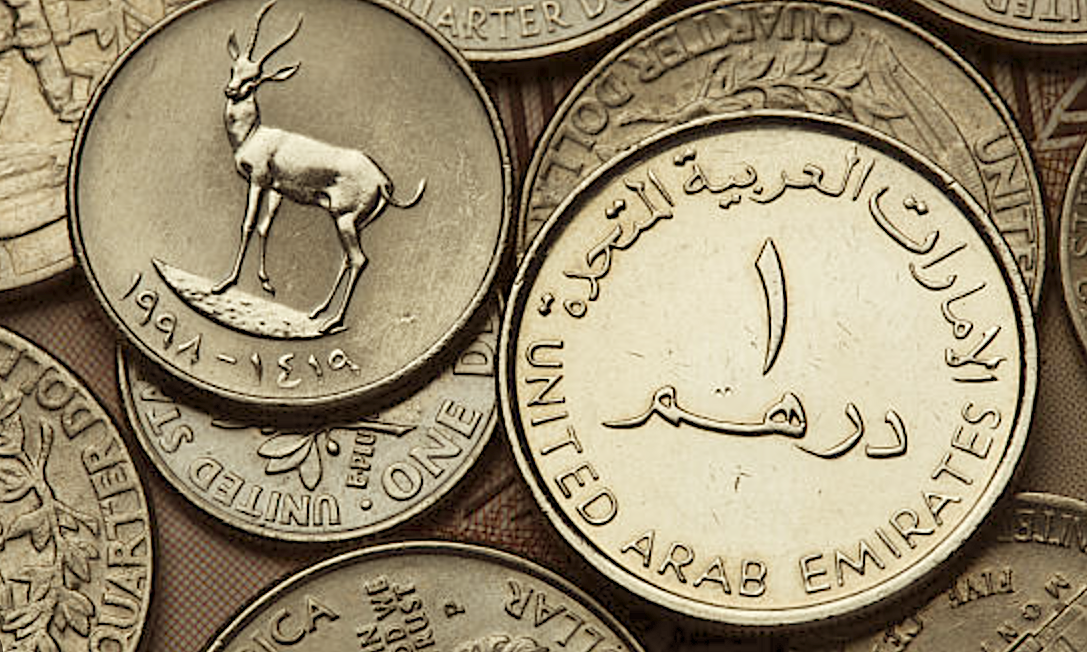
\includegraphics[scale=.2]{figs/coin.png} \\
\vspace{.5in}
\pause
{\tiny
 Solution:  
 a) $\frac{{6 \choose 2}}{2^6}$, b)  $\frac{1}{2^6}$ c)  $1- \frac{1}{2^6}$
 
 
  }
\end{frame}





\begin{frame}
\vspace{-.15in}
\qBrd[4.65in]{purple!30}{ \Exmpl{purple!50}{} A fair-dice is thrown 8 times and all the the 8 numbers  that appear are recorded.  
\begin{enumerate}[a).]
\qBrd[4in]{applegreen!40}{ \item What is the probability that there is  no $\HLTW{Six}$?}
\qBrd[4in]{babyblue!40}{ \item What is the probability that there is at least one $\HLTW{Six}$?}
\qBrd[4in]{amber!40}{ \item What is the probability that there will  be exactly 3 $\HLTW{Four}$'s and 2 $\HLTW{Three}$'s among the eight throws?}
\end{enumerate}
\vspace{.05in}
} 

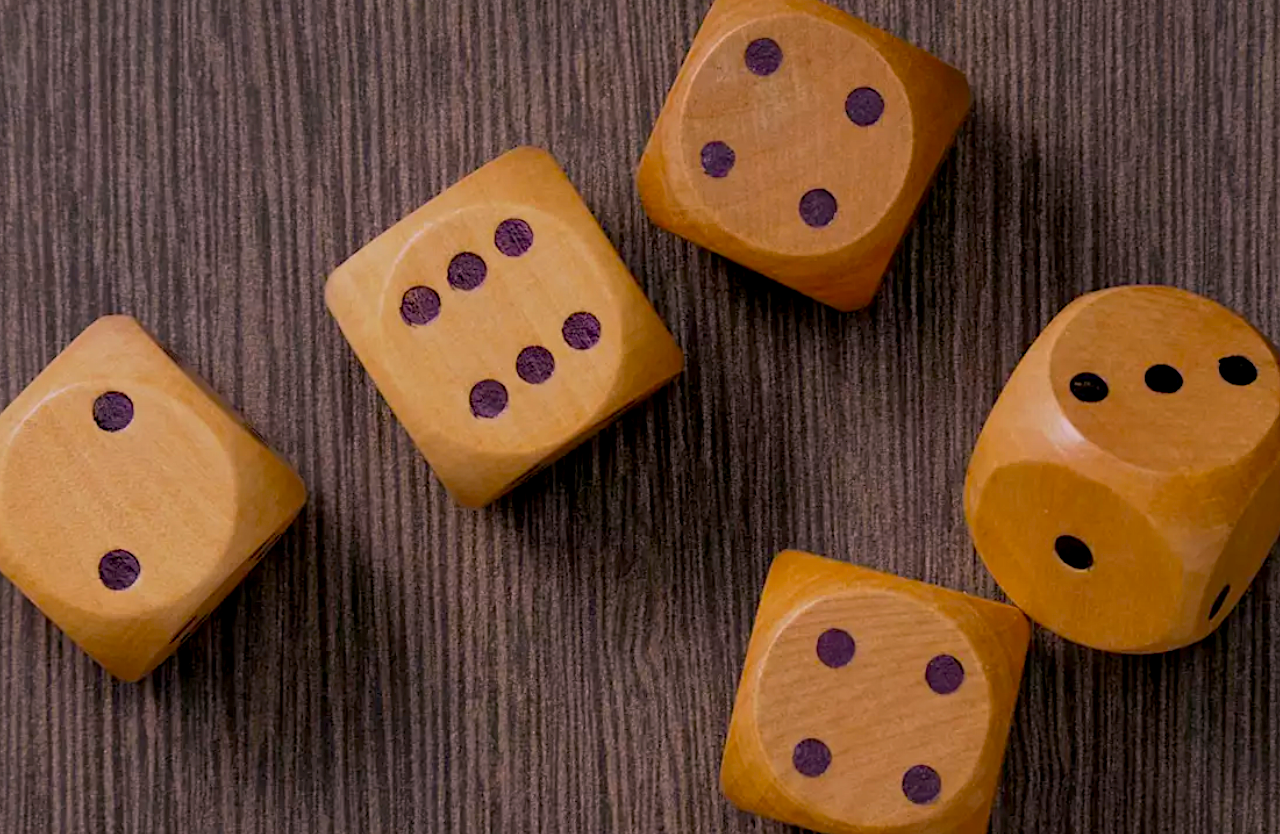
\includegraphics[scale=.15]{figs/dice.png} \\
\vspace{.1in}
\pause
{\tiny Solution: 
a) $\frac{5^8}{6^8}$, b) $1-\frac{5^8}{6^8}$, c) $ \frac{{ 8 \choose 3  }{ 5 \choose 2  } 4^3 }{6^8}  $
}

\end{frame}






%
%\begin{frame}\frametitle{Example}
%\qbx[4.5in]{applegreen!40}{
%\Exmpl{applegreen}{} If 3 balls are randomly drawn from a bowl
%containing 6 white and 5 black balls, what is the probability
%that one of the balls is white and the other two black?
%}\\
%\pause
%\vspace{1.5in}
%{\tiny Solution: $n=11 \times 10\times 9 = 990$ and $n(E)=?$ if
%$E=\{\text{one of the balls is white and the other two black}\}$
%For the order WBB we have $6 \times 5 \times 4=120$
%possibilities, for BWB, we have $5 \times 6 \times 4=120$ possibilities and for BBW we have $ 5\times 4 \times 6=120$
%possibilities. Then $P(E)=\frac{n(E)}{n}=\frac{ 120+120+120}{990} = \frac{4}{11}$.}
%\vspace{2in}
%
%\end{frame}




\begin{frame}
\qbx[4.5in]{teal!40}{\Exmpl{teal}{}
One of the sections in the class STAT230 has 10 students.  Assume the birthday of a student can be any one of days out of 365 days in a year.  We say that the two students share a same birth day if they are born on the same day and same month {\tiny ( for example two students are born on $10^{\text{th}}$ January).}  Answer the following questions. 
\begin{enumerate}[a).]
\item What is the probability that there are exactly four students who have the same birthday?
\item What is the probability that at least two of the students have the same birthday?
\end{enumerate} 
}\\
\vspace{.8in}
\pause
{\tiny
 Solution:\\
  a)   $\frac{365\times  {10 \choose 4} \times ^{364}P_{6}}{365^{10}}= \frac{365\times  {10 \choose 4} \times 364\times 363 \times 362 \times 361 \times 360 \times  359}{365^{10}}$\\
  b)  $1- \frac{^{365}P_{10}}{365^{10}}$ }
 \vspace{.11in}
\end{frame}




%
%\begin{frame}\frametitle{Example}
%\qbx[4.5in]{darksalmon!40}{
%\Exmpl{darksalmon}{} A committee of 5 is to be selected from a group of 6 men and 9 women.  If the selection is made randomly, what is the probability that the committee consists of 3 men and 2 women?
%}\\
%\pause
%\vspace{1.5in}
%{\tiny {\bf Solution: } \\
% Because each of the ${15 \choose 5}$ possible committees is equally likely to be selected, the desired
%probability is $\frac{{6 \choose 3}\times {9 \choose 2}}{{15 \choose 5}}=0.24$}
%\vspace{1in}
%
%\end{frame}
%
%
%


\begin{frame}
\qbx[4.5in]{amber(sae/ece)!40}{\Exmpl{amber(sae/ece)}{} 
A typical ATM pin consists of 4 digits.  Assume that all the integers between $0$ to $9$ are equally likely for selecting each of the digits. Find the probability of the following events. 
\begin{enumerate}
\item What is the probability that all the four digits of a randomly selected ATM pin is different?
\item *The bank has selected a group of 120 ATM users randomly.  What is the probability that atleast two of the users have exact same ATM pin? {\tiny Assume that all the possible four digit numbers  are equally likely to be considered as a PIN of a randomly selected user. }
\item *What would be corresponding probability if 300 ATM users are  randomly chosen instead?
\end{enumerate}  }\\

\begin{minipage}{.45\textwidth}
\includegraphics[scale=.25]{figs/ATMPIN.png} 
\end{minipage}
\begin{minipage}{0.45\textwidth}
\pause
{\tiny
 Solution:  
 a) $\frac{^{10}P_4}{10^4}$ \\
 
 b)  $1- \frac{^{^{10000}}P_{_{120}}}{10000^{^{120}}}\approx 0.5117 $, \\
 
 c)  $1- \frac{^{10000}P_{300}}{10000^{300}}\approx 0.9892 $ }
\end{minipage}


%\pause 
\vspace{.5in}

\end{frame}





\begin{frame}\frametitle{}
Suppose that there is 6 identical balls and they are to be distributed among three kids,  Ayesha, Abdullah, and Anawar  ({\tiny consider the scenario when a kid may obtain NONE,One or More balls}).  
\begin{enumerate}
\item What is the probability that Ayesha receievd exactly two balls?\\
\item  What is the probability that Ayesha receievd at least  one ball?\\
\end{enumerate}

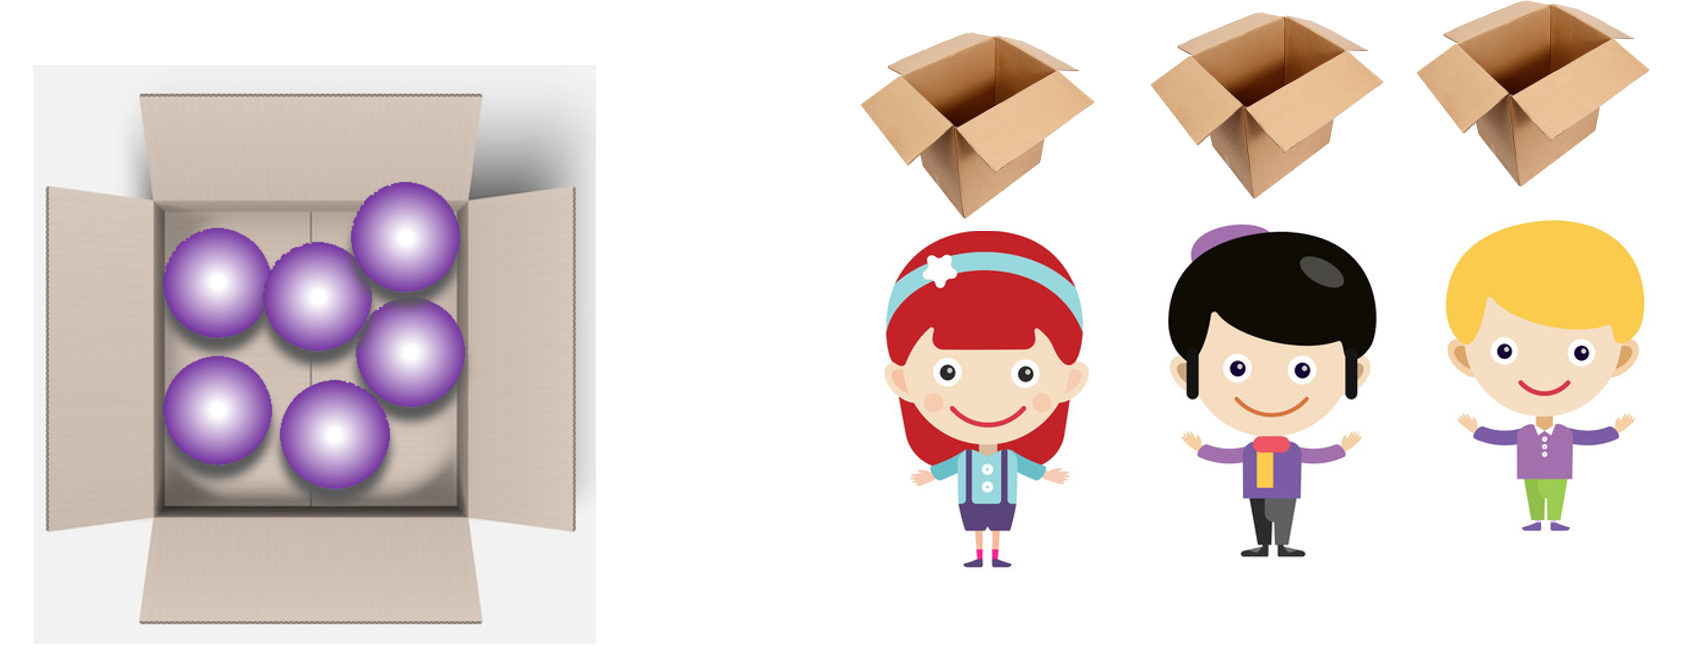
\includegraphics[scale=.32]{figs/6PurpleBass3kids.png}


\pause
{\tiny Solution: 
\begin{itemize}
\item $\frac{ {{4+2-1}\choose {2-1} } }{ {{6+3-1}\choose {3-1}}  }$\item $1- \frac{ {{6+2-1}\choose {2-1} } }{ {{6+2-1}\choose {2-1}}  }$
\end{itemize} 
}
\vspace{.5in}
\end{frame}





%
%
%\begin{frame}
%\qbx[4.5in]{teal!40}{\Exmpl{teal}{} 
%A student prepares for an exam by studying a list of {\bf ten problems}.  She only practiced {\bf six of them}. For the examination, the instructor selects {\bf five problems} at random from the ten on the list given to the students.  What is the probability that the student can solve all five problems on the exam?  }\\
%
%{\tiny
% Solution:  }
%%\pause 
%\vspace{2in}
%
%\end{frame}






%
%\begin{frame}\frametitle{Example}
%\qbx[4.5in]{darkraspberry!40}{
%\Exmpl{darkraspberry}{} Suppose 5 people are to be randomly selected from a group of 20 individuals consisting of 10 married couples, and we want to determine $P(N)$, the probability that the 5 chosen are all unrelated. (That is, no two are married to each other.)
%}\\
%\pause
%\vspace{1.5in}
%{\tiny 
%Solution: 
%$P(N)=\frac{{10 \choose 5}\times 2^5}{{20 \choose 5}}\implies P(N)=\frac{20 \times 18\times 16\times 14\times 12}{20\times 19\times 18\times 17\times 16}$
%}
%\vspace{2in}
%
%\end{frame}
%

%
%
%\begin{frame}\frametitle{Example}
%\qbx[4.6in]{darktangerine!40}{
%\Exmpl{darktangerine}{} If $n$ people are present in a room, what is the probability that no two of them celebrate their birthday on the same day of the year? How large need n be so that this probability is less than $\frac{1}{2}$?
%}\\
%\pause
%\vspace{1.5in}
%{\tiny 
%Solution: 
%$\frac{^{365}P_n}{(365)^n}=\frac{(365)\times (364) \times \cdots \times (365-n+1)}{(365)^n}$
%}
%\vspace{2in}
%
%\end{frame}



%
%\begin{frame}\frametitle{Example}
%\qbx[4.5in]{cherryblossompink!40}{
%\Exmpl{cherryblossompink}{}A poker hand consists of 5 cards. If the cards have distinct consecutive values and are not all of the same suit, we say that the hand is a straight. For instance, a hand consisting of the five of spades, six of spades, seven of spades, eight of spades, and nine of hearts is a straight.  What is the probability that one is dealt a straight?
%}\\
%\pause
%\vspace{1.5in}
%{\tiny 
%Solution: 
%?
%}
%\vspace{2in}
%
%\end{frame}


\begin{frame}
\begin{center}
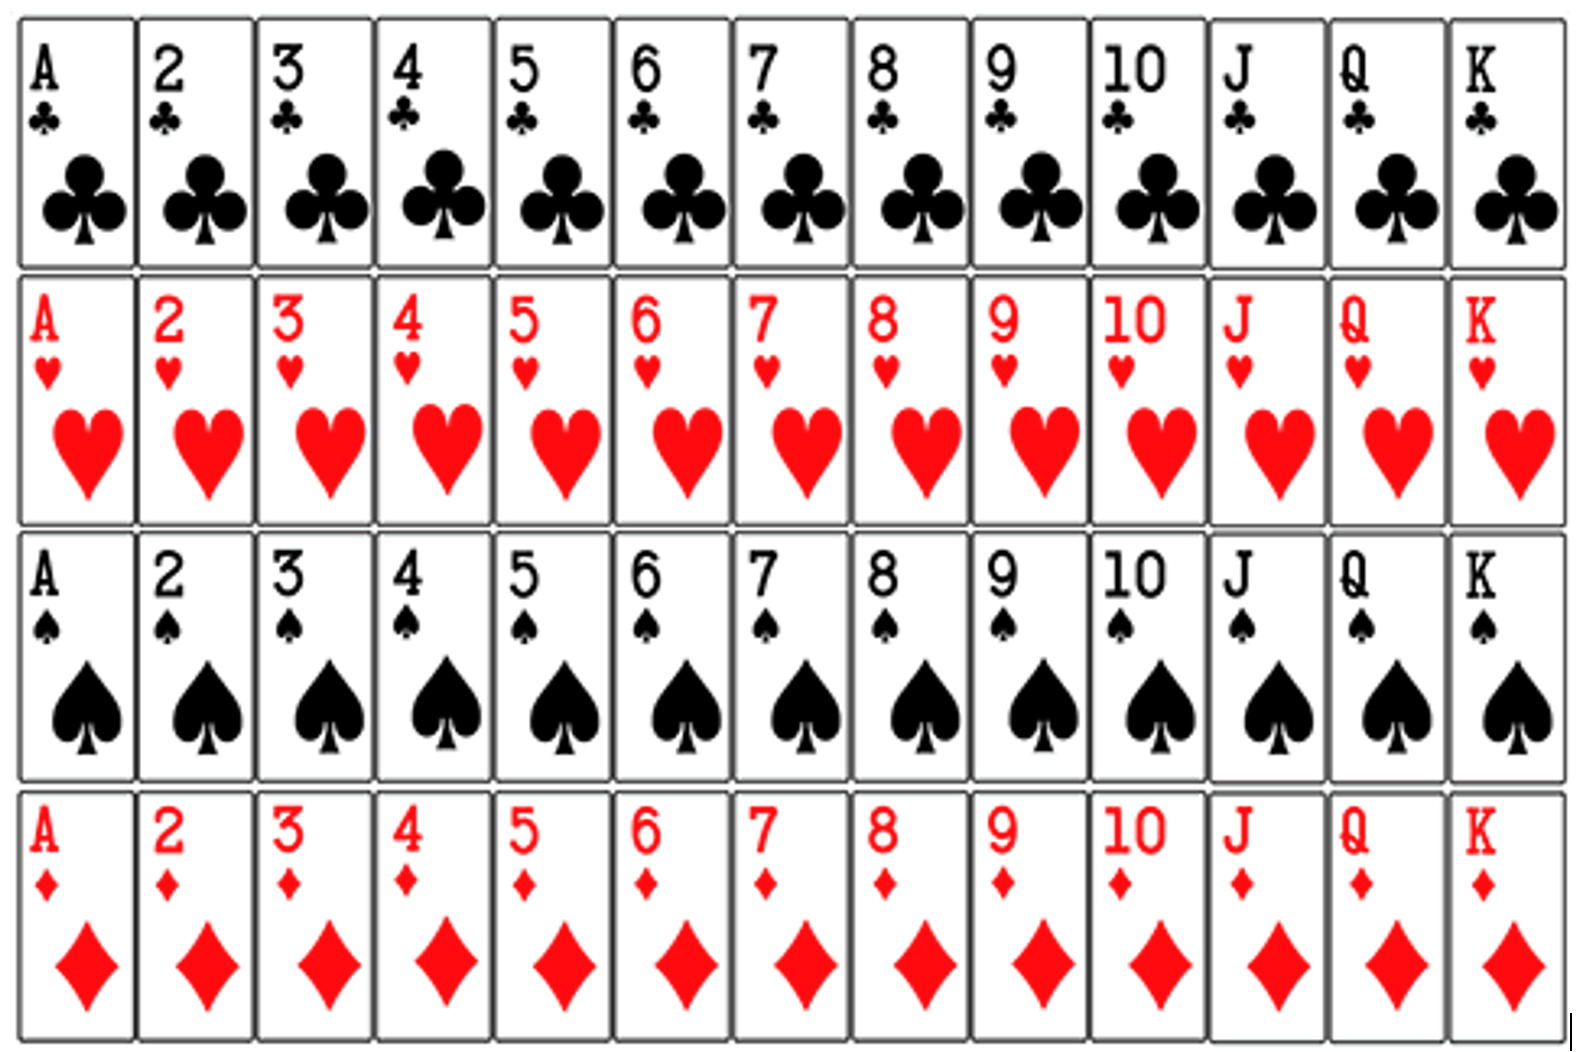
\includegraphics[scale=.4]{figs/Cards.png}
\end{center}
\end{frame}



\begin{frame}
\qbx[4.5in]{capri!40}{
\small 
\Exmpl{capri}{} In the game of bridge, the entire deck of 52 cards is dealt out to 4 players.  A card is selected randomly from the deck.
\begin{enumerate}[a).]
\item What is the probability that  the cards is an `Ace'?
\item What is the probability that  the cards is either a  `King' or a 'Queen'? 
\end{enumerate}
}\\
\begin{center}
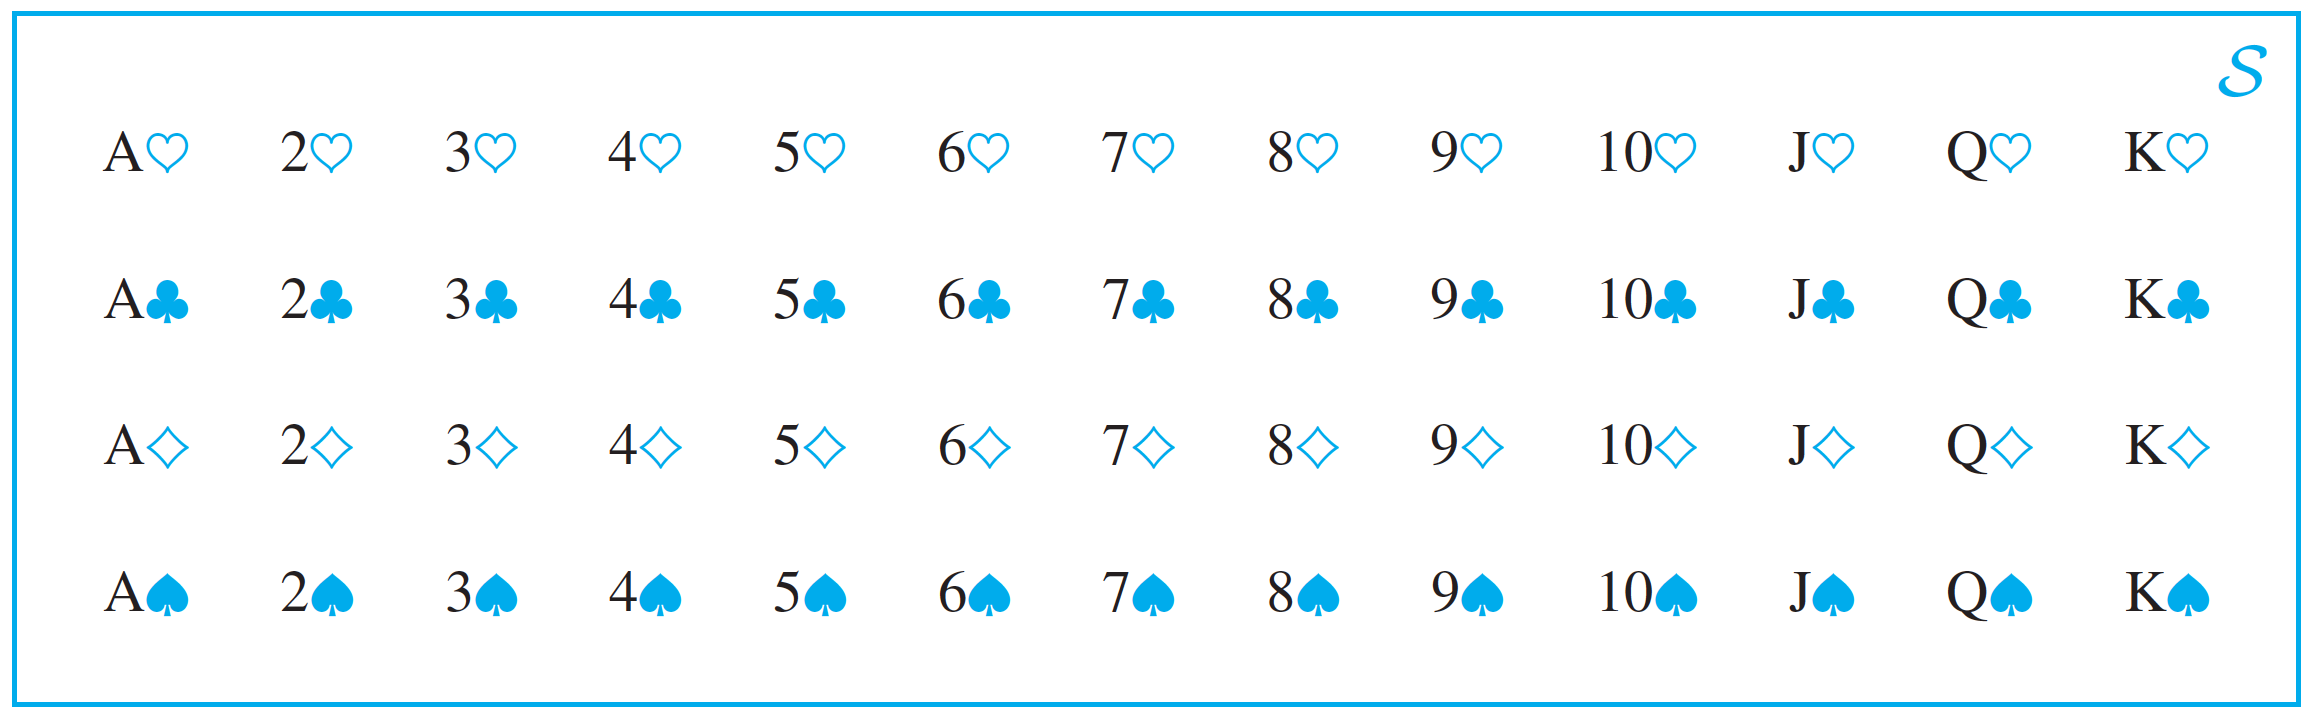
\includegraphics[scale=.27]{figs/Cards_Sample.png}
\end{center}
\vspace{1in}
\end{frame}




\begin{frame}
\qbx[4.5in]{slateblue!40}{
\small 
\Exmpl{slateblue}{} Two cards are selected randomly from the deck of 52 cards.
\begin{enumerate}[a).]
\item What is the probability that both the cards are  `Ace's?
\item What is the probability that at least one of them is an Ace?
\end{enumerate}
}\\
\begin{center}
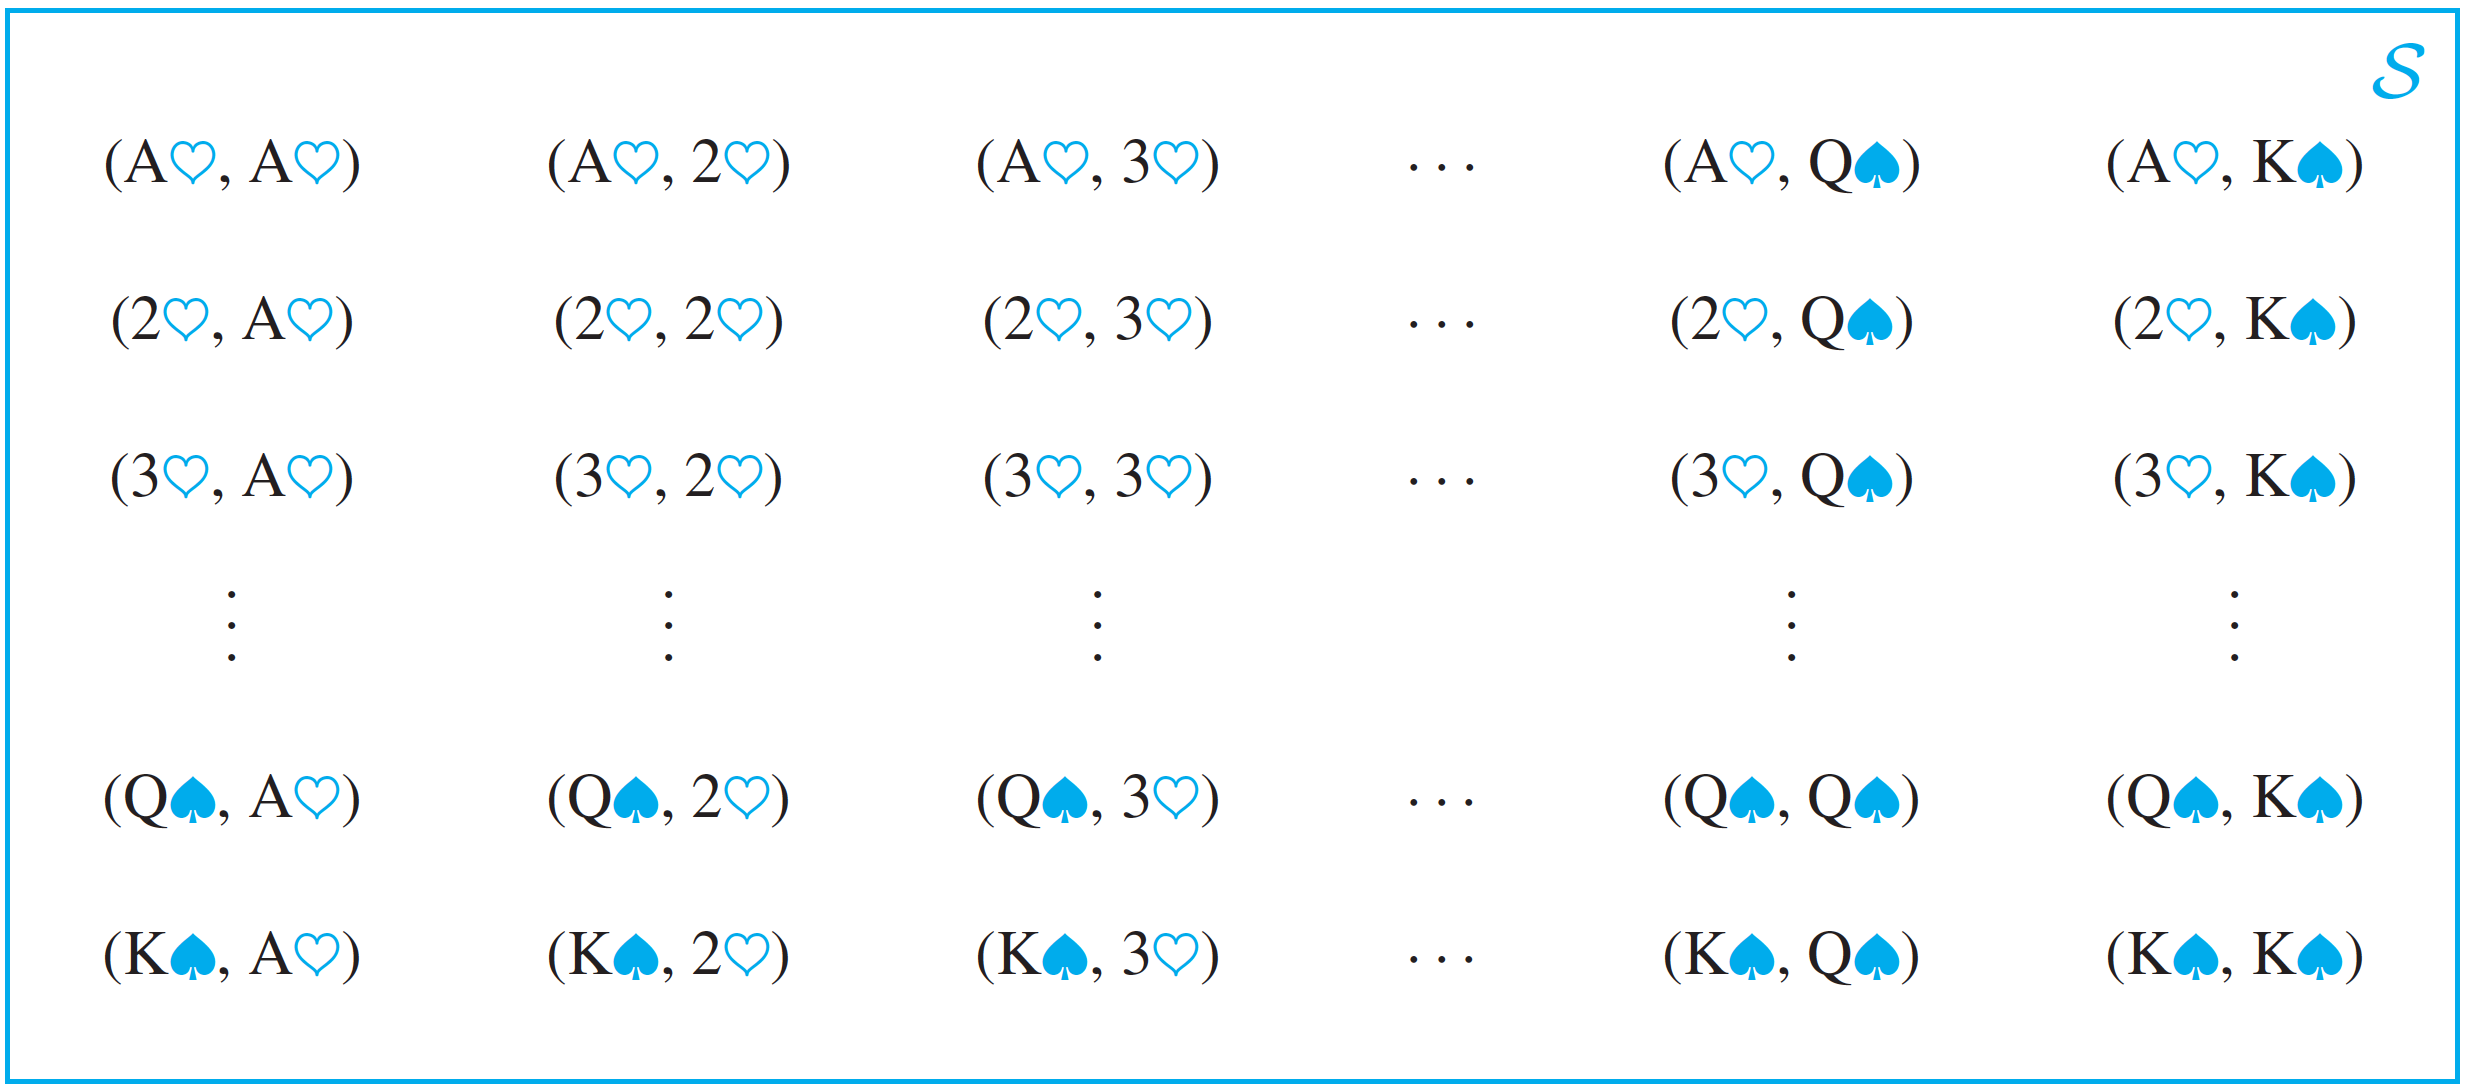
\includegraphics[scale=.25]{figs/Cards_two_sample.png}
\end{center}
\vspace{1.5in}
\end{frame}


\begin{frame}\frametitle{Example}
\qbx[4.5in]{bluebell!40}{
\Exmpl{bluebell}{} In the game of bridge, the entire deck of 52 cards is dealt out to 4 players. What is the probability that
\begin{enumerate}[a).]
\item one of the players receives all 13 spades?
\item each player receives 1 ace?
\end{enumerate}
}\\
\pause
\vspace{1in}
{\tiny  Solution: 

a) $ \frac{   {4 \choose 1}\times  { 13 \choose 13} \times { 39 \choose {13,13,13}}    }{  {52 \choose {13,13,13,13}} }  =  \frac{   {4 \choose 1}\times  1 \times  \frac{39!}{ {13! \times 13! \times 13!}}   } {  \frac{52!}{{13!\times 13!\times 13! \times 13!}} } =   \frac{   {4 \choose 1}\times 39! \times 13! } { 52!} $ whcih is also same as $\frac{4}{{52\choose 13}} $.
\vspace{.1in}
b) $\frac{4! {48 \choose {12, 12, 12, 12}} }{{52 \choose {13,13,13,13}}}$
}
\vspace{2.5in}

\end{frame}



%
%
%\begin{frame}\frametitle{Example}
%\qbx[4.5in]{airforceblue!40}{
%\Exmpl{airforceblue}{} A pack of 52 playing cards always plays a key role in probability concept. Whenever we go through the stuff probability in statistics, we will definitely have examples with a well shuffled pack of 52 playing cards. 
%\begin{enumerate}[a).]
%\item What is the probability that one player get one ?
%\item each player receives 1 ace?
%\end{enumerate}
%}\\
%\pause
%\vspace{1in}
%{\tiny 
%Solution: 
%
%a) $ \frac{   {4 \choose 1}\times  { 13 \choose 13} \times { 39 \choose {13,13,13}}    }{  {52 \choose {13,13,13,13}} }  =  \frac{   {4 \choose 1}\times  1 \times  \frac{39!}{ {13! \times 13! \times 13!}}   } {  \frac{52!}{{13!\times 13!\times 13! \times 13!}} } =   \frac{   {4 \choose 1}\times 39! \times 13! } { 52!} $ whcih is also same as $\frac{4}{{52\choose 13}} $.
%
%b) $\frac{4! {48 \choose {12, 12, 12, 12}} }{{52 \choose {13,13,13,13}}}$
%}
%\vspace{2.5in}
%
%\end{frame}
%



%\begin{frame}{ Examples: On Sharing a Birthday  }
%
%\qBox{\Qn:
%There are 15 students registered in the course STAT320.  What is the probability that at least two of the students will share their Birthday? (Ignore the leap year and assume there is 365 days in a year) 
%}
%
%
%\pause
%\vspace{1.5in}
%{\tiny Solution: 
%$P(\{\text{At least two students have same birthday}\})=1-P(\text{None of the students have same birthday})=1-\frac{365\times 364\times \ldots \times 351}{365^{15}}\approx 1-0.7470987=0.25  $
%}
%
%
%\end{frame}




\begin{frame}{De-arrangement: Application of Inclusion Exclusion Principle}
\qBox{\Exmpl{blue!30}{} Suppose we turn over cards simultaneously from two well shuffled decks of ordinary playing cards. We say we obtain an exact match on a particular turn if the same card appears from each deck; for example, the queen of spades against the
queen of spades.  Let $C_i$ denotes the event that there is an exact match at the $i^{\text{th}}$ turn.   
\begin{enumerate}[a).]
\item Argue that   $\HLTW{P(C_i)=\frac{51!}{52!}}.$ 
\item  Argue that  for $\HLTW{i_i\neq i_2 $,  $P(C_{i_1} \cap C_{i_2})= \frac{50!}{52!}}$. 
\item  Argue that  for $\HLTW{i_1\neq i_2 \neq i_3 $,  $P(C_{i_1} \cap C_{i_2} \cap C_{i_3})= \frac{49!}{52!}}$. 
\item Show that the  probability of at least one exact match is 
$\HLTW{ 1-\frac{1}{2!}+\frac{1}{3!}-\frac{1}{4!}+\cdots -\frac{1}{52!}}$.
\end{enumerate}
}
%\qBox{\Qn:
%Find the number of nonnative integer solutions of $X_1, X_2, X_3, $  such that $X_1+X_2+X_3=14$. \\
%\HLT[yellow]{Ans: 120}
%}
%
%\qBox{\Qn:
% Consider an Experiment,  where a  dice is thrown 4 times.
%Calculate the probability that the sum of all the through is 17?
%}
\vspace{1in}
\end{frame}






\begin{frame}{Application of Inclusion Exclusion Principle}
\qBrd[4.6in]{amethyst!50}{\Exmpl{amethyst!30}{} Suppose that there is a practice session for a UAE football (soccer) team.   In that session all the 11 players randomly picked up a jersey from a basket where exactly 11 jerseys were kept.  Note that, all the jerseys have the players name written on it, therefore in the basket there were exactly one jersey that would match with a specific player.  What is the probability that none of the players have picked up the jersey that would match their name?
}
%\qBox{\Qn:
%Find the number of nonnative integer solutions of $X_1, X_2, X_3, $  such that $X_1+X_2+X_3=14$. \\
%\HLT[yellow]{Ans: 120}
%}
%
%\qBox{\Qn:
% Consider an Experiment,  where a  dice is thrown 4 times.
%Calculate the probability that the sum of all the through is 17?
%}
\vspace{1in}
\end{frame}



\TransitionFrame[antiquefuchsia]{\Large Questions?  }
 
 
\end{document}
